%-------------------------------------------------------------------------------
% TEYSSIER Maxime
% IUT Béziers - LP Réseaux et Télécommunications Parcours IdO 
% Promotion: 2018/2019
% Stage IUT de Béziers
% Intitulé: WalkersVision
% Tuteur: DRUON Sebastien
%-------------------------------------------------------------------------------

%-------------------------------------------------------------------------------
% Titre du fichier
%-------------------------------------------------------------------------------
\title{Rapport_WalkersVision}

%-------------------------------------------------------------------------------
% Fonctionnalités
%-------------------------------------------------------------------------------
\documentclass[12pt, french]{report}
\usepackage[a4paper]{geometry}
\usepackage[myheadings]{fullpage}
\usepackage[french]{babel}
\usepackage[T1]{fontenc}
\usepackage[utf8]{inputenc}
\usepackage{sectsty}
\usepackage[font=small, labelfont=bf]{caption}
\usepackage{fourier}
\usepackage[protrusion=true, expansion=true]{microtype}
\usepackage{fancyhdr}
\usepackage{lastpage}
\usepackage{graphicx, wrapfig, subcaption, setspace, booktabs}
\usepackage{titletoc}
\usepackage{hyperref}
\usepackage{tikz}
\usepackage{multicol}
\usepackage{xcolor}
\usepackage{color}
\usepackage{url}
\usepackage{minted}
\onehalfspacing
\setcounter{tocdepth}{5}
\setcounter{secnumdepth}{5}
\renewcommand{\thesection}{\arabic{section}}
\newcommand{\HRule}[1]{\rule{\linewidth}{#1}}
\definecolor{LightGray}{gray}{0.7}
\usepackage{tikz}
\usepackage{amsmath}
\usepackage{pdfpages} 
\usepackage{pdflscape}
\usepackage{biblatex}
\bibliographystyle{plain} 
\bibliography{bibli.bib}

%-------------------------------------------------------------------------------
%Début du document
%-------------------------------------------------------------------------------
\begin{document}

%-------------------------------------------------------------------------------
% En-tête & pied de page
%-------------------------------------------------------------------------------
\pagestyle{fancy}
\fancyhf{}
\setlength\headheight{15pt}
\fancyhead[L]{Maxime TEYSSIER}
\fancyhead[R]{IUT de Béziers}
\fancyfoot[R]{Page \thepage\ sur \pageref{LastPage}}

%-------------------------------------------------------------------------------
% Page de garde
%-------------------------------------------------------------------------------

\title{
\includegraphics[width=0.56\textwidth]{Images/IUT-Beziers.png}\\
		\normalsize\textsc{}
		\HRule{2pt} \\
        \LARGE \textbf{\uppercase{Rapport de stage\\Comptage et statistiques de passants sur une place publique par analyse}}
		\HRule{2pt} 
		\normalsize 04 Juin 2019 - 27 Août 2019 \vspace*{3\baselineskip}
        }
\author{Stagiaire: Maxime TEYSSIER\\Tuteur: Sébastien DRUON\\ 
        
\includegraphics[width=0.25\textwidth]{Images/UM.png}
        \date{}\\
        }
\maketitle
\clearpage
\newpage
%%%%%%%%%%%%%%%%%%%%%%%%%%%%%%%%%%%%%%%%%%%%%%%%%%%%%%%%%%%%%%%%%%%%%%%%%%%%%%%
%%%%%%%%%%%%%%%%%%%%% Page blanche sans mise en page %%%%%%%%%%%%%%%%%%%%%%%%%%
%%%%%%%%%%%%%%%%%%%%%%%%%%%%%%%%%%%%%%%%%%%%%%%%%%%%%%%%%%%%%%%%%%%%%%%%%%%%%%%
\strut
\thispagestyle{empty}
\newpage
%%%%%%%%%%%%%%%%%%%%%%%%%%%%%%%%%%%%%%%%%%%%%%%%%%%%%%%%%%%%%%%%%%%%%%%%%%%%%%%
\thispagestyle{empty}							      

%----------------Remerciements--------------------------------------------------
\section*{Remerciements}
J'adresse mes remerciements aux personnes qui m'ont permis à réaliser ce stage au sein de l'IUT de Béziers.\\

En premier lieu, M. Sébastien DRUON, professeur de l'Institut Universitaire de Technologie de Béziers, pour m'avoir donné l'opportunité de faire ce stage et de m'avoir accepté au sein de son équipe. Mais aussi en qualité de tuteur d'entreprise, en me guidant dans mon travail et m'aider lors de difficultés.\\

Je souhaite remercier M. Frédéric COMBY, professeur de l'Institut Universitaire de Technologie de Béziers, pour m'avoir aidé lors de difficultés rencontré.\\

Je tiens à remercier aussi l'équipe de l'Institut Universitaire de Technologie de Béziers, pour leur sympathie et leur gentillesse apporté durant ce stage.\\

\newpage

\renewcommand{\thepage}{}
%-------------------------------------------------------------------------------
%-------------------------------------------------------------------------------
% Sommaire								       
%-------------------------------------------------------------------------------
\tableofcontents
\clearpage 

%-------------------------------------------------------------------------------
% Début des écrits
%-------------------------------------------------------------------------------

%%%%%%%%%%%%%%%%%%%%%%%%%%%%%
\startcontents[mainsections]%
%%%%%%%%%%%%%%%%%%%%%%%%%%%%%

\newpage
\renewcommand{\thepage}{\arabic{page}}
\setcounter{page}{1}

\section{Introduction}
\setcounter{page}{1} 
    % Mise en explication du sujet
    % Identification du besoin
    % Modelisation du terrain 


% A la recherche d'une intro
    % 1/
    \begin{itemize}
        \item "Les recensements de population constituent la source principale des études sociodémographiques portant sur le local, et en particulier sur le niveau infra communal, celui des quartiers. Ils permettent des descriptions des caractéristiques du peuplement des quartiers sous l’aspect structurel en appréciant les écarts avec leur environnement proche, par exemple celui de la commune ou de l’unité urbaine à laquelle ils appartiennent."
        (Source: \href{https://www.cairn.info/revue-francaise-des-affaires- sociales-2001-3-page-39.htm}{https://www.cairn.info/revue-francaise-des-affaires- sociales-2001-3-page-39.htm})\\
        

    % 2/
    \item "Le domaine de vision par ordinateur, poussé par les progrès scientifiques et technologiques récents, s’oriente vers l’analyse en temps réel des scènes comportant des sujets humains." (Source: \href{https://tel.archives-ouvertes.fr/tel-00004804/document}{https://tel.archives-ouvertes.fr/tel-00004804/document} ) %- titre / auteur: Vision par ordinateur pour l’interaction homme-machine fortement couplée - De François Bérard - Thèse) \\
    \\
    \end{itemize}
        
    Ce rapport de stage de Licence Professionnelle de Réseaux et Télécommunication porte sur le thème de la fréquentation d'une place dans la ville de Béziers. Le domaine de la vision par ordinateur nous permet d'obtenir de multiples résultats en temps réel. C'est pour cela que, pour analyser comme le demande la mission, un ordinateur recevant des images pourra en déduire les informations que nous lui demanderons. \\
    Tout au long de ce rapport, nous allons comprend ce qu'est une image et comment la traiter. Par la suite nous allons faire des mathématiques théorique pour comprendre le fonctionnement de la vision stéréo et l'appliqué. \\
    Pour réaliser ce stage, j'ai utilisé la librairie OpenCV et j'ai programmé en langage C/C++.

\newpage
\section{Présentation}
\subsection*{L'établissement}

L'Institut Universitaire de Technologie de Béziers propose des formations universitaires alliant théorie et pratique qui répondent aux attentes des entreprises en termes de formation technologique. \\

Depuis 2011, l’IUT de Béziers s’est installé dans ses nouveaux locaux, place du 14 juillet. Proche du centre-ville, il s’inscrit parfaitement dans la vie de ce quartier qui accueille déjà la Médiathèque André Malraux, l’antenne Du Guesclin de l’Université Paul-Valéry et le Centre interrégional de développement de l’occitan.\\

\textbf{Directeur}: Philippe Pujas\\

\textbf{Directrice administrative}: Annie Molès\\
\bigskip

\textbf{Quelques chiffres}\\
\begin{itemize}
        \item 510 étudiants en formation continue, 49 en apprentissage
        \item 3 départements d'enseignement: Réseaux et Télécommunications, Métiers du Multimédia et de l'Internet, Techniques de commercialisation
        \item Plus de 100 partenaires entreprises\\
\end{itemize} 


\textbf{Contact}:\\ 3, Place du 14 juillet,\\ BP 50438,\\ 34505 Béziers cedex\\ Tél.: +33(0)4 67 11 60 00


\subsection*{La mission}
    
Le stage a pour but d'être utile pour la ville de Béziers. La mission est une solution qui créer des statistiques de passants sur une place public. \\

La mission est, dans un premier temps, de connaître le nombre de passants sur la place en temps réel. Les données traitées seront envoyés vers un serveur via TCP/IP ou LoRa. Seul des données transiterons. Aucune image sera transmise.\\ 

Dans un second temps, nous essayerons de remonter l'endroit ou ce trouve les passants sur la place et connaître leur typologie (adulte/enfant).\\

De plus, un dimensionnement de caméra est à réaliser.


\subsection*{Horaires}

\begin{center}
        \begin{tabular}{|l|l|l|l|l|c|r|}
                \hline
                Lundi & Mardi & Mercredi & Jeudi & Vendredi \\
                \hline
                9h00 - 12h00 & 09h00 - 12h00 & 9h00 - 12h00 & 9h00 - 12h00 & 9h00 - 12h00 \\
                \hline
                PAUSE&PAUSE&PAUSE&PAUSE&PAUSE\\
                \hline
                13h00 - 17h00 & 13h00 - 17h00 & 13h00 - 17h00 & 13h00 - 17h00 & 13h00 - 17h00 \\ 
                \hline
        \end{tabular}
\end{center}
\newpage

\newpage
%%%%%%%%%%%%%%%%%%%%% Page blanche avec mise en page %%%%%%%%%%%%%%%%%%%%%%%%%%
\strut									      %
\newpage							              %
%%%%%%%%%%%%%%%%%%%%%%%%%%%%%%%%%%%%%%%%%%%%%%%%%%%%%%%%%%%%%%%%%%%%%%%%%%%%%%%
\newpage

\section{Traitement d'image}
Avant de traiter une image, qu'est ce qu'une image? Une image est une matrice de valeurs. Les valeurs diffèrent de la propriété de l'image. Lorsque je vais prendre une image elle aura des valeurs qui définit les couleurs sur un espace de couleur BGR (Blue - Green - Red).\\

Par exemple, cette icône:\\
\begin{center}
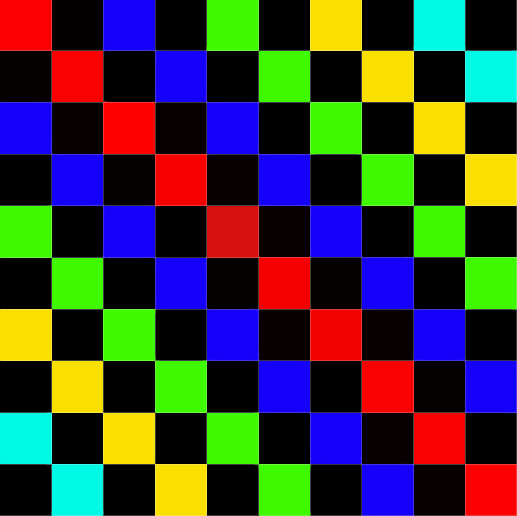
\includegraphics[width=3cm,heigth=3cm]{Images/iconeGrande.PNG}\\
\textit{icone - 10x10 pixels}
\end{center}

A pour données:


\begin{minted}[
    baselinestretch=1.4,
    bgcolor=lightgray,
    fontsize=\footnotesize]
{bash}

[1,1,252,0,0,4,249,0,21,0,0,0,0,249,62,0,0,0,0,224,249,0,0,0,229,249,0,0,0,0;
1,1,6,1,1,250,0,0,0,249,0,21,0,0,0,0,249,62,0,0,0,0,224,249,0,0,0,229,249,0;
249,0,21,1,1,8,0,0,254,0,0,6,249,0,21,0,0,0,0,249,62,0,0,0,0,224,249,0,0,0;
0,0,0,249,0,21,1,1,6,0,0,247,1,1,7,249,0,21,0,0,0,0,249,62,0,0,0,0,224,249;
0,249,62,0,0,0,249,0,21,0,0,1,15,15,215,1,1,9,249,0,21,0,0,0,0,249,62,0,0,0;
0,0,0,0,249,62,0,0,0,249,0,21,1,1,6,1,1,245,1,1,6,249,0,21,0,0,0,0,249,62;
0,224,249,0,0,0,0,249,62,0,0,0,249,0,21,0,0,8,1,1,242,1,1,7,249,0,21,0,0,0;
0,0,0,0,224,249,0,0,0,0,249,62,0,0,0,249,0,21,0,0,0,1,1,250,1,1,6,249,0,21;
229,249,0,0,0,0,0,224,249,0,0,0,0,249,62,0,0,0,249,0,21,1,1,7,1,1,248,0,0,0;
0,0,0,229,249,0,0,0,0,0,224,249,0,0,0,0,249,62,0,0,0,249,0,21,1,1,7,1,1,252]

\end{minted}

L'interprétation pour ce cas est que l'image est en BGR ( Blue Green Red). Donc les données affichés sont par paquets de 3 valeurs (vecteur de 3). Le premier pixel par exemple a pour valeur [1,1,255], qui vaut la couleur ROUGE.

        \subsection{Ouvrir et afficher une image}
                Une image peut être enregistrer sur un disque sous format .jpg, .png... Dans ce cas là, une fonction nous permettra de charger l'image. Pour cela nous utiliserons "imread()". Cela dit, via une webcam nous pouvons prendre une photo et la charger. Pour cela, nous utiliserons la fonction "VideoCapture". Deux choix sont possible: utiliser une image déjà créer ou prendre une photo.


                \subsubsection{"imread"}
                Le fonction \textit{imread()} va nous servir pour traiter dans un premier temps une image enregistré sur le disque.
                L'image en question est Lena ou Lenna.
                Cette photo est un standart dans le test d'image pour deux raison selon David C. Munson, éditeur en chef lors des discussions de l'IEEE sur le traitement d'image de janvier 1996: 
                "Tout d'abord, cette image contient un mélange intéressant de détails, de régions uniformes, et de textures, ce qui permet de bien tester les différents algorithmes de traitement d'image. C'est une bonne image de test ! Ensuite, « Lenna » est l'image d'une femme attirante. Ce n'est pas une surprise que la communauté de la recherche dans le traitement d'image (principalement masculine) gravite autour d'une image qu'elle trouve attirante." 
                \begin{center}
                        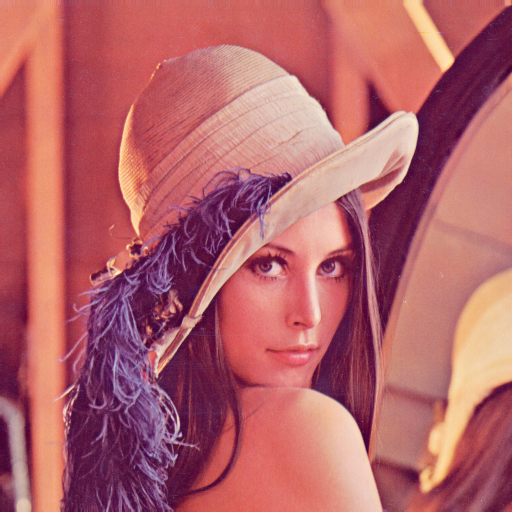
\includegraphics[width=0.4\textwidth]{Images/Lenna.png}\\
                        \textit{Photo 1 - Lenna}\\
                \end{center}

                \begin{minted}[
                    baselinestretch=1.4,
                    bgcolor=LightGray,
                    fontsize=\footnotesize]
                    {c++}
#include <opencv2/opencv.hpp>
using namespace cv;
int main(int argc, char** argv ){
    if ( argc != 2 ){ //Si le nombre d argument dépasse 2 (le prog+le nom de l image)
        printf("usage: programme <Image_Path>\n");// Affichage message
        return -1; // ERROR
    }
    Mat image; // Stocke les donnees de l image dans la tableau de classe Mat
    image = imread( argv[1], 1 ); // Charge la matrice que l'image represente
    if ( !image.data ){// Si la matrice n'a pas de valeur
        printf("No image data \n");
        return -1; // ERREUR
    }
    namedWindow(argv[1], WINDOW_AUTOSIZE ); // On nomme une fenêtre 
    imshow(argv[1], image); //Affiche l'image dans la fenêtre 
    waitKey(0); // Attend une action via une touche pour quitter
    return 0;
}
                \end{minted}
                \begin{center}
                    \textit{Programme 1 - Chargement d'une image et affichage}\\
                \end{center}
                
                Résultat après compilation et exécution: 
                \begin{center}
                        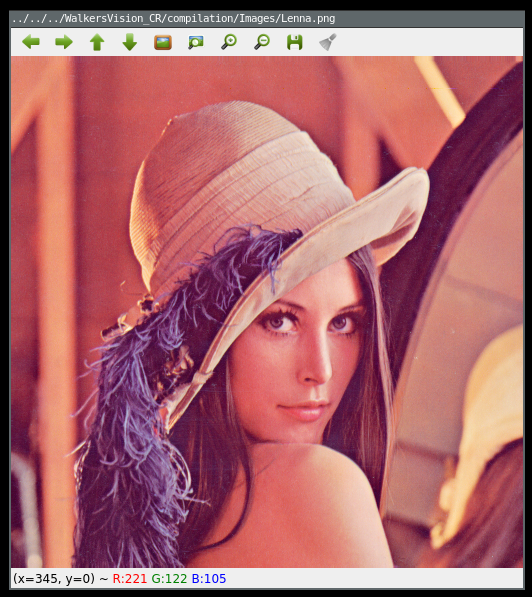
\includegraphics[width=0.5\textwidth]{Images/PrintImageSimple.png}\\
                        \textit{Résultat 1 - Affichage d'une image chargé}
                \end{center}

                \subsubsection{"VideoCapture"}
                La fonction \textit{VideoCapture} nous permet de prendre une instantanée via une caméra.
                \begin{minted}[
                    baselinestretch=1.4,
                    bgcolor=LightGray,
                    fontsize=\footnotesize]
                    {c++}

#include "opencv2/opencv.hpp"
using namespace cv;
int main (int argc, char **argv){
  VideoCapture camera(atoi (argv[1])); // Ouvre la caméra demandé en argument
  if (!camera.isOpened ()){return -1;}
      Mat image;
      camera >> image;	// Récupère l'image / matrice depuis la caméra
      imshow ("Webcam", image); // Affiche l'image
      waitKey (0)
  return 0;
}
               \end{minted}
               \begin{center}
                   \textit{Prise d'instantanée depuis caméra et affichage}
               \end{center}

                Résultat après compilation et exécution: 
               \begin{center}
                   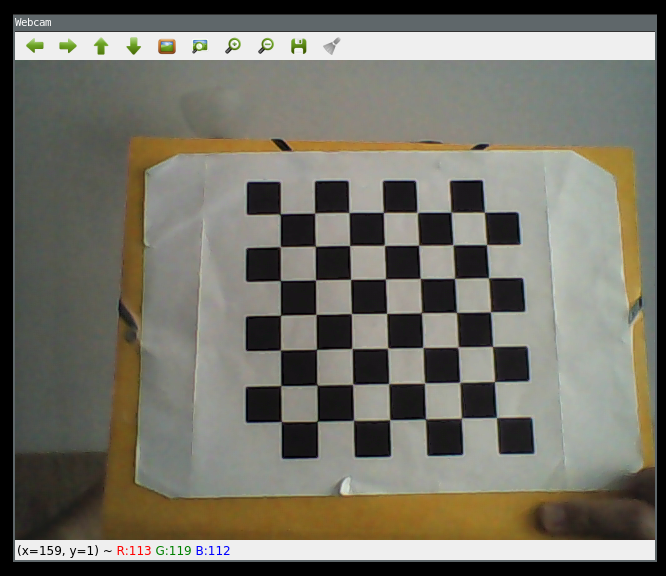
\includegraphics[width=0.5\textwidth]{Images/PhotoWebcam.png}\\
                   \textit{Résultat 2 - Prise d'instantanée et affichage}
               \end{center} 
                

        \subsection{Changement d'espace de couleur}
            Le changement d'espace de couleur permet de voir différemment la même image et ainsi la traiter avec plus d'efficacité. Voici deux espace de couleur différente à BGR, les différentes luminances de gris et les teintes-saturation-valeur (HSV).
            Pour effectuer ce changement, l'utilisation de la fonction \textit{cvtColor()} sera utile.
                \subsubsection{BGR2GRAY}
                Voici un code qui permet de passer de l'espace de couleur BGR en celui de gris: 
                
                \begin{minted}[
                    baselinestretch=1.4,
                    bgcolor=lightgray,
                    fontsize=\footnotesize]
                    {c++}
#include <opencv2/opencv.hpp>
using namespace cv;
int main(int argc, char ** argv){
        char * imageName = argv[1]; // on recupère le chemin où est l'image
        Mat image;
        image =imread(imageName);
        if(argc!=2 || !image.data){
                printf("ERROR");
                return -1;
        }
        Mat gray_image;
        // cvtColor(source, destination, traduction d'espace de couleur)
        cvtColor(image, gray_image, COLOR_BGR2GRAY); 
        imshow(imageName, image);
        imshow("Gray image", gray_image);
        waitKey(0);
        return 0;
}
                \end{minted}
                
                \begin{center}
                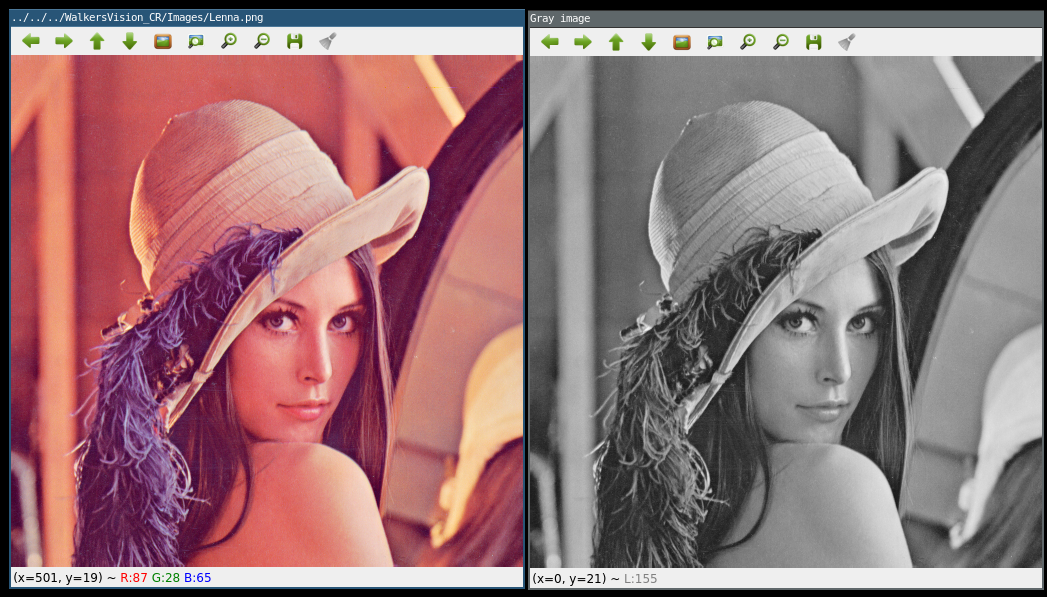
\includegraphics[width=0.8\textwidth]{Images/ImgBGR2GRAY.png}\\
                \textit{Résultat 3 - Affichage image normal et teinte de gris}
                \end{center}


                \subsubsection{BGR2HSV}
                Pour notre mission de compter des passants, nous avons besoin de reconnaître un humain d'un arbre ou bâtiment. Dans l'espace de couleur HSV (Hue, Saturation, Value) à la différence d'autres espaces de couleurs, tout les humains ont la même teinte (Hue).
                Pour changer l'espace BGR en HSV, le code est le quasi le même que précédent sauf un paramètre dans \textit{cvtColor}:\\
                
                \begin{minted}[
                 baselinestretch=1.4,
                bgcolor=lightgray,
                fontsize=\footnotesize]
                {c++}
#include <opencv2/opencv.hpp>
using namespace cv;
int main(int argc, char ** argv){
        char * imageName = argv[1]; 
        Mat image;
        image =imread(imageName);
        if(argc!=2 || !image.data){ printf("ERROR"); return -1;}
        Mat hsv_image;
        cvtColor(image, hsv_image, COLOR_BGR2HSV); 
        imshow(imageName, image);
        imshow("Lena HSV", hsv_image);
        waitKey(0);
        return 0;
}
                \end{minted}

                \begin{center}
                 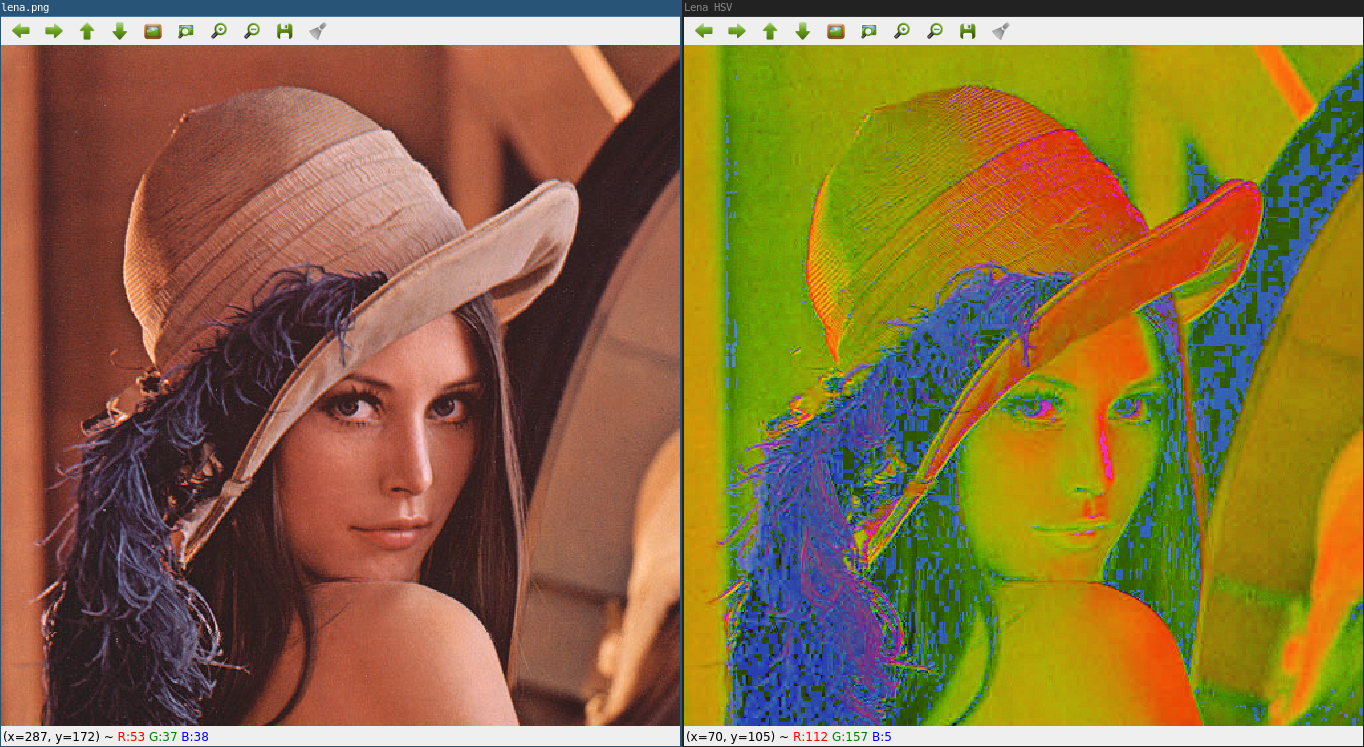
\includegraphics[width=0.8\textwidth]{Images/BGR2HSV.png}\\
                 \textit{Traduction d'espace BGR en HSV}
                \end{center}
                
                
        \subsection{Capturer la peau humaine}
        Pour capturer la peau humaine sur une image, le traitement de l'image par l'espace de couleur HSV est possible. Pour cela, il faut définir une plage de couleur (dans l'espace HSV) à garder. Ainsi, l'extraction affichera la peau humaine.\
        
        \begin{minted}[
        baselinestretch=1.4,
        bgcolor=lightgray,
        fontsize=\footnotesize]
        {c++}
#include <opencv2/opencv.hpp>
using namespace cv;
using namespace std;
int main (int argc, char *argv[]){
    Mat frame, frame_HSV, frame_threshold, PH;
    frame =imread(argv[1], IMREAD_COLOR);
    PH = frame.clone (); 
    cvtColor (frame, frame_HSV, COLOR_BGR2HSV, 0);
    // Création d'une plage de valeurs pour identifier la peau
    inRange (frame_HSV, Scalar (1, 3, 150), Scalar (9, 147, 240),
	       frame_threshold);
    for (int i = 0; i < PH.rows; i++){
	    for (int j = 0; j < PH.cols; j++){
	        // L'image apparaît en noir ou blanc à la comparaison des pixels
	        // de l'image 'frame_threshold'. L'opération consiste à modifier
	        // les pixels de l'image 'PH' lorsque 'frame_threshold'
	        // a pour pixel la valeur différente de blanc.
	        if (frame_threshold.at < unsigned char >(Point (j, i)) != 255){
		        PH.at < Vec3b > (Point (j, i)) = Vec3b (0, 0, 0);
		    }
	    }
	}
    imshow ("Image Traite", PH);
    imshow ("Image", frame);
    waitKey(0); 
    return 0;
}
    \end{minted}
                
    \begin{center}
        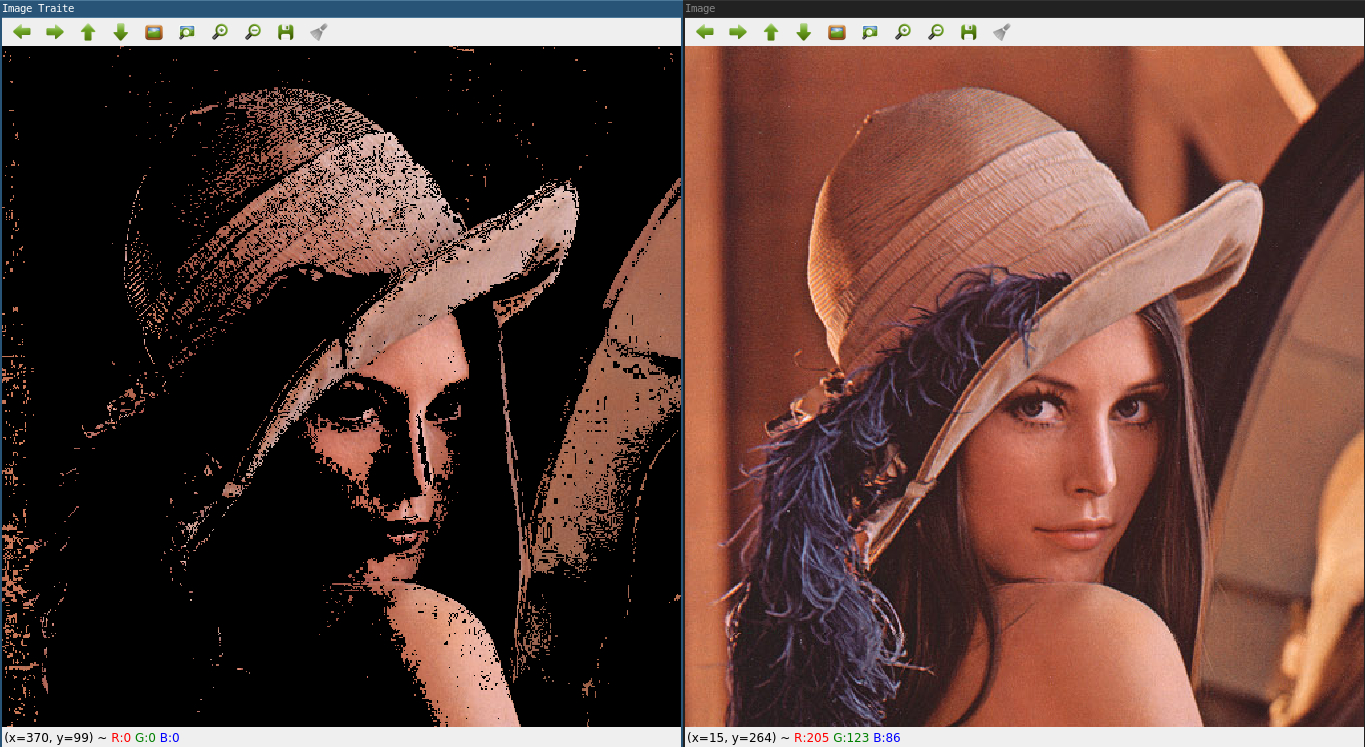
\includegraphics[width=0.8\textwidth]{Images/CPH.png}\\
        \textit{Capture de la peau humaine avec des parasites}
    \end{center}

    Le traitement ne permet pas d'avoir un résultat parfait. Pour améliorer le filtre, l'utilisation de dilatation et érosion de pixel est une méthode possible.\\
    
    \subsection{Suppression de fond}
    \subsubsection{MOG2}
    
    Sur l'étape précédente, le résultat nous affiche le fond d'une image alors que le résultat devrait être juste la peau humaine. Cela dit, si la couleur est dans la même tranche de valeur accepté que celle demandé l'objet va apparaître sur l'image. 
    Pour y remédier, la suppression de fond est nécessaire. Pour la réalisation, l'utilisation d'une vidéo est exigé car le programme ci-dessous, permet de supprimer tout ce qui ne bouge pas, soit le fond. 
    
    \begin{minted}[
    baselinestretch=1.4,
    bgcolor=lightgray,
    fontsize=\footnotesize]
{c++}
#include "opencv2/imgcodecs.hpp"
#include "opencv2/imgproc.hpp"
#include "opencv2/videoio.hpp"
#include <opencv2/highgui.hpp>
#include <opencv2/video.hpp>
#include <stdio.h>
#include <iostream>
#include <sstream>
using namespace cv;
using namespace std;

Mat frame,fgMaskMOG2; 
Ptr<BackgroundSubtractor> pMOG2; 
int keyboard; 
void processWcam(char* videoFilename){
    VideoCapture capture(atoi(videoFilename));
    if(!capture.isOpened()){exit(EXIT_FAILURE);}
    while( (char)keyboard != 'q'  && (char)keyboard != 27 ){
        if(!capture.read(frame)) {exit(EXIT_FAILURE);}
        GaussianBlur(frame,frame,Size(5,5),0,0); // Ajout de flou
        GaussianBlur(frame,frame,Size(5,5),0,0);
        pMOG2->apply(frame, fgMaskMOG2);
        stringstream ss;

        imshow("Frame", frame);
        imshow("FG Mask MOG 2", fgMaskMOG2);
        keyboard = waitKey(30);
    }
    capture.release();
}
int main(int argc, char* argv[]){
    while(true){
            pMOG2 = createBackgroundSubtractorMOG2(); 
            processWcam(argv[1]);
            destroyAllWindows();
            return EXIT_SUCCESS;
        }
}

\end{minted}
    
    \begin{center}
        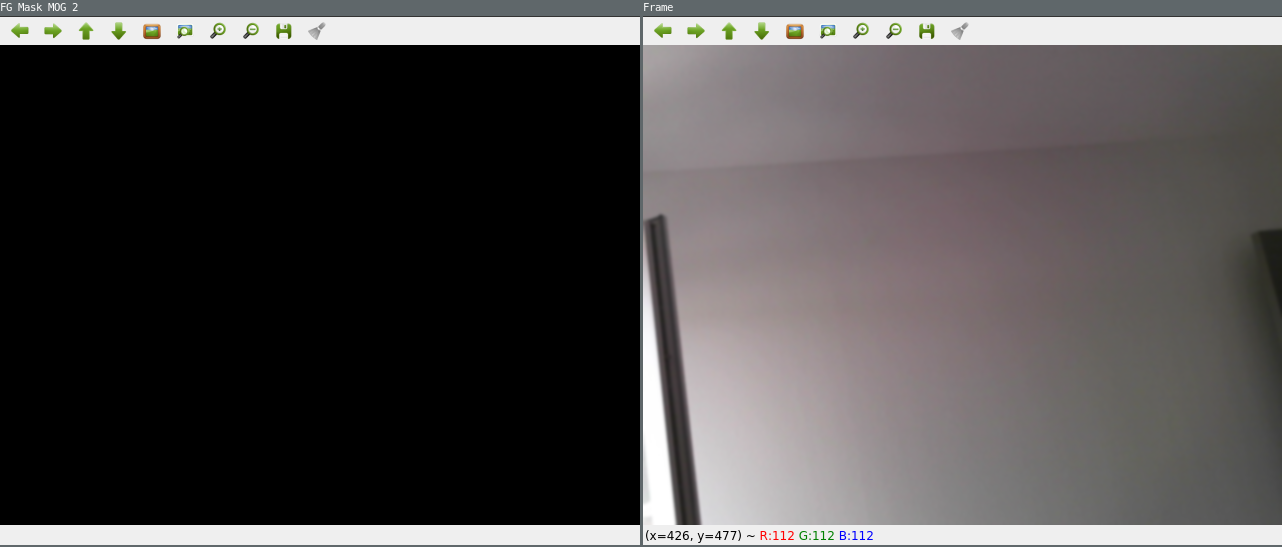
\includegraphics[width=0.8\textwidth]{Images/BGSub/BGSub0.png}\\
        \textit{Suppression du fond lors d'aucun mouvement}
    \end{center}
    
    \begin{center}
        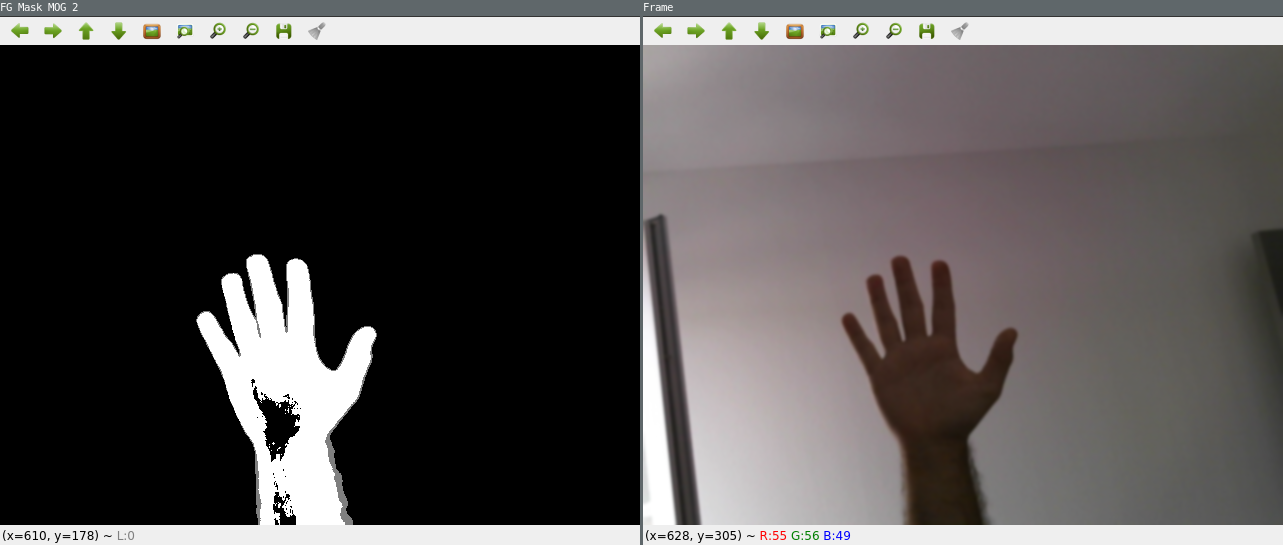
\includegraphics[width=0.8\textwidth]{Images/BGSub/BGSub1.png}\\
        \textit{Suppression du fond lors d'un mouvement}\\
    \end{center}    
    
    Via ce programme, le résultat est donné sur un seuil (threshold). Si les valeurs exactes des pixels ne sont pas affiché cela devient un problème pour la suite. C'est à dire, nous avons un résultat en noir et blanc. nous ne pourrons pas traiter la couleur avec ce résultat.
    
    \subsubsection{Pixel par pixel}
    Pour avoir un maximum de détail, le résultat doit ressortir les couleurs. Donc, le programme suivant va afficher les pixels réel au lieu de pixel blanc sur l'ancien programme.
    
    \begin{minted}[
    baselinestretch=1.4,
    bgcolor=lightgray,
    fontsize=\footnotesize]
{c++}
#include "../../opencv/imgproc.hpp"
#include "../../opencv/core.hpp"
#include "../../opencv/highgui.hpp"
#include "../../opencv/opencv.hpp"
#include <iostream>
#include <cmath>
using namespace cv;
using namespace std;
// Calcul permet de de faire filtre de couleur et donner une moyenne pour
// garantir que le pixel est bien le fond ou non
int Calcul(unsigned char a, unsigned char b, unsigned char c, unsigned char d,
           unsigned char e, unsigned char f ){
    int A,B,C,D,E,F,r;
    A=(int)a; B=(int)b; C=(int)c ; D=(int)d; E=(int)e; F=(int)f; r=abs((B-E)+(C-F));
    if ((A>3) && (A<14) && (B>40) && (B<190) && (C>100) && (C<250) && 
        (A-D<10) && (B-E<10) && (C-F<10) ){ 
        return r;
    } else {
        r=0;
    }
}
int main(int argc, char **argv){
    int renew=0;
    unsigned char R,G,B,H1,S1,V1,H,S,V,Res,Bes,Ges;  
    VideoCapture cap(atoi(argv[1]));
    Mat webcam, whsv(480,640,CV_8UC3), reference,rhsv(480,640,CV_8UC3),
        resultat(480,640,CV_8UC3), ero,dil;
    cap>>reference;
    cvtColor(reference,rhsv,COLOR_BGR2HSV);// Passage HSV

    while(true){
        while(renew==2){ // Rafraîchir l'image de référence
            cap>>reference;
            GaussianBlur(reference,reference,Size(5,5),0,0);
            GaussianBlur(reference,reference,Size(5,5),0,0);
            GaussianBlur(reference,reference,Size(5,5),0,0);
            erode(reference,reference,Mat(),Point(1,1),2,1);
            cvtColor(reference,rhsv,COLOR_BGR2HSV);// Passage HSV
            renew=0;
        }
        cap>>webcam;
        GaussianBlur(webcam,webcam,Size(5,5),0,0); // ajout de flou
        GaussianBlur(webcam,webcam,Size(5,5),0,0); // 5x5 pixels
        GaussianBlur(webcam,webcam,Size(5,5),0,0);
        cvtColor(webcam,whsv,COLOR_BGR2HSV); // Passage HSV
        if(!cap.isOpened()){cout << "Error opening video stream or file"
                                                        << endl;return -1;}
        for(int i=0;i<480; i++){// Rows 
            Vec3b *ptr = webcam.ptr<Vec3b>(i) ; // WebCam
            Vec3b *ptrwhsv = whsv.ptr<Vec3b>(i) ; // Webcam HSV
            Vec3b *ptrrhsv = rhsv.ptr<Vec3b>(i) ; // Reference HSV
            Vec3b *ptres = resultat.ptr<Vec3b>(i) ; // Resultat
            for(int j=0;j<640;j++){ // Cols
                H=ptrwhsv[j](0); // h webcam 
                S=ptrwhsv[j](1); // s webcam
                V=ptrwhsv[j](2); // v webcam
                H1=ptrrhsv[j](0); // H reference
                S1=ptrrhsv[j](1); // S reference
                V1=ptrrhsv[j](2); // V reference
                int A= Calcul(H,S,V,H1,S1,V1); 
                if( A>1) {
                    // Affichage de pixel réel
                    ptres[j](0)=ptr[j](0);
                    ptres[j](1)=ptr[j](1);
                    ptres[j](2)=ptr[j](2);
                }else{ // Sinon pixel -> Noir
                    ptres[j](0)=0;
                    ptres[j](1)=0;
                    ptres[j](2)=0;
               }
            }
        }
       imshow("Reference", rhsv);
       imshow("Resultat", resultat);
        if(waitKey(30)>=0){break;}
        renew++;
    }
    cap.release();
    return 0;
}
\end{minted}
    
    \begin{center}
        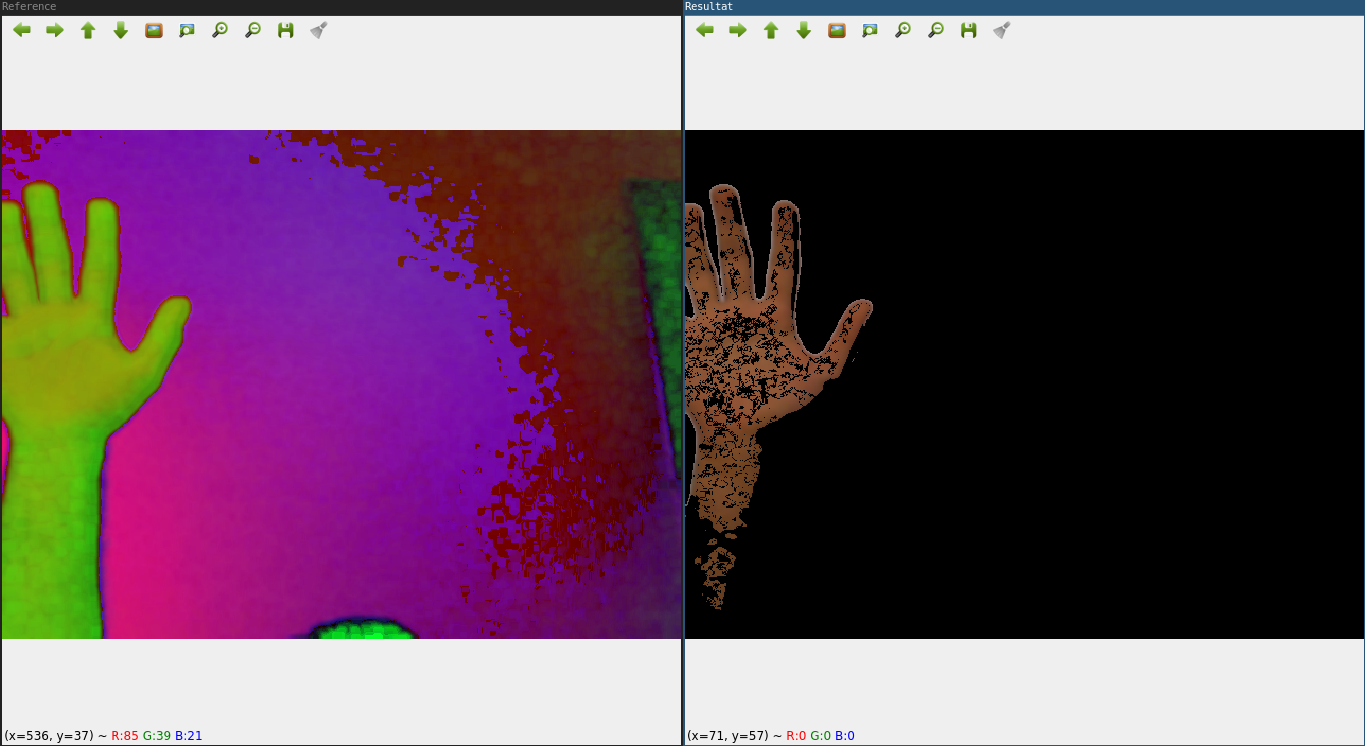
\includegraphics[width=0.8\textwidth]{Images/BGSub/BGSubWithColor.png}\\
        \textit{Suppression du fond et affichage de la couleur original des pixels}
    \end{center}
    \subsection{Conclusion}
    
    Cette partie a permis de voir ce qu'est une image en informatique, une matrice. De celle ci, on a pu l'afficher dans une fenêtre en tant qu'image et on a pu afficher une succession d'image, une vidéo. De plus, le fait d'analyser et pouvoir traiter ses données de chaque image, donne accès à modifier ses valeurs. Ainsi, changer l'espace de couleur de BGR en HSV est devenu possible pour nous. De ce fait, la création de filtre pour accepter qu'un intervalle de valeurs pour identifier la peau humaine devient possible. Dans le même cas, la suppression du fond par analyse de pixel est créé. 
    \newpage
%%%%%%%%%%%%%%%%%%%%%%%% CAMERA %%%%%%%%%%%%%%%%%%%%%%%%%%%%
\section{Caméra}
\subsection{Calibration - théorie}
\subsubsection{Vision}
Lorsque l'on prend une photo, le capteur perçoit un point sur un plan 2D (2 dimension).\\

\begin{center}
    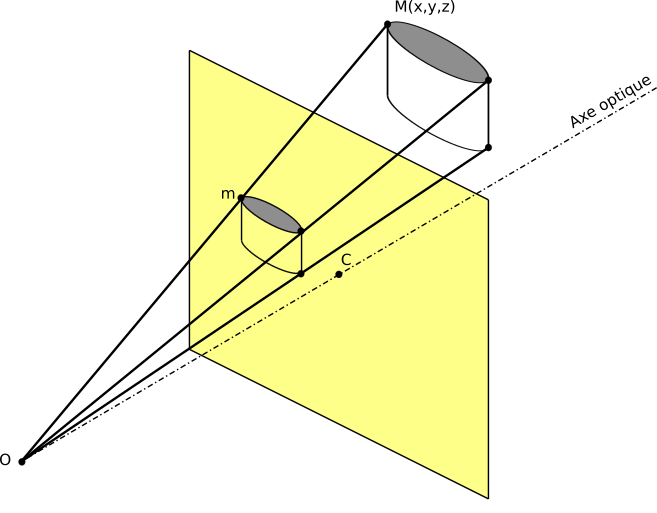
\includegraphics[width=0.8\textwidth]{Images/Vision/Projection2D.png}
\end{center}



Le schéma ci-dessous présente un plan orthonormé en 3D, avec comme axes X, Y et Z. Lorsque l'on inscrit un pixel sur une image, par exemple "m", nous avons pris la valeur du point M sur ses axes x et y car le capteur n'a pas de notion de profondeur, qui est la dimension manquante, la Z.

\begin{center}
    \begin{tikzpicture}
    \path(0,-0.2) node{O};
    \path(0,2.2) node{Y};
    \path(2.2,-0.5) node{Z};
    \path(1.5,1.7) node{X};
    \path(8,2.3) node{M(X,Y,Z)};
    \path(3.9,1.3) node{m};
    \path(3.9,0.98) node{x};
    % Repere 0
    \draw[->](0,0) -- (2,-0.5); % Axe Z
    \draw[->](0,0) -- (1.5,1.5); % Axe X
    \draw[->](0,0) -- (0,2); % Axe Y
    % Image perçu
    \draw[-](3,-2)--(3,2); % Gauche
    \draw[-](3,2)--(5,4) ;% Haut
    \draw[-](5,4)--(5,0) ;% Droit
    \draw[-](5,0)--(3,-2); % Bas
    % Exemple de perception d'un point sur une image
    \draw[-](0,0) -- (8,2); % Vecteur M 
    \draw(8,2) circle (0.05); % Vecteur M 
    \end{tikzpicture}
\end{center}

Le point \textbf{M} à pour valeur x,y,z. Que l'on écrit: $$\textbf{M}\begin{bmatrix}x\\y\\z\end{bmatrix}$$

Sur un plan en 2D (Hauteur[Y]/Profondeur[Z]), nous avons:\\

\begin{center}
    \begin{tikzpicture}
    \path(0,-0.2) node{O};
    \path(0,2.2) node{Y};
    \path(6.15,0) node{Z};
    \path(-0.2,0.2) node{X};
    \path(7,1.5) node{M(x,y,z)};
    \path(3.4,0.4) node{V};
    \path(5.7,0.75) node{y};
    \path(1.5,-1) node{f}; % f
    \path(2.75,-2) node{z}; % f
    \path(2.7,1) node{m(u,v)}; % f
    \path(3,0.75) node{x}; % f
    %%%%%%%%%%%%%%%%%%%%%%%%%%%%%%%%%%
    \draw[->](0,0) -- (6,0); % Axe Z
    \draw[->](0,0) -- (0,2); % Axe Y
    \draw[-](0,0) -- (6,1.5); % Vecteur M
    \draw (6,1.5) circle (0.05);
    %%%%%%%%%%%%%%%%%%%%%%%%%%%%%%%%%%%
    \draw[-,dashed](3,-1) -- (3,2); % Barre V
    \draw[-,dashed](5.5,-2) -- (5.5,2); % Barre Y
    \draw[<->](0,-0.65) -- (3,-0.65); % Barre f 
    \draw[<->](0,-1.5) -- (5.5,-1.5); % Barre z
    \end{tikzpicture}
\end{center}
Ce point de vue nous permet d'appliquer le théorème de Thalès pour récupérer des informations. Nous pouvons effectuer : $\frac{v}{y}$ = $\frac{f}{z}$ \\

Ainsi on peut en déduire de : $v=\frac{fY}{z}$ et $u=\frac{fX}{Z}$

\subsubsection{Erreur de centrage}

Nous pouvons écrire la matrice: 
$$\left\{ 
    \begin{array}{ll}
        v=\frac{fY}{Z}+V0  \\ \\
        u=\frac{fX}{Z}+U0
    \end{array} \\
\right. $$ \\

Que l'on peut écrire: 
$$\left\{ 
    \begin{array}{ll}
        v=\frac{fY+V0Z}{Z} \\ \\
        u=\frac{fX+U0Z}{Z}
    \end{array} \\
\right. $$

La préférence de coordonnée homogène nous fait écrire le système:
$$\left\{ 
    \begin{array}{ll}
        v'=fY+U0\\ \\
        u'=fX+U0 \\ \\
        w'=Z
    \end{array} \\
\right. $$

Avec ces nouvelles forme d'écriture nous écrivons: $u=\frac{u'}{w'}$ et $v=\frac{v'}{w'}$

\subsubsection{Matrice de projection}
Ainsi la matrice s'écrit:
$$\begin{matrix}
    
    \underbrace{\begin{bmatrix}
        u'\\v'\\w'\\
    \end{bmatrix}}_{\text{Coord. H. pixel}}
    
    =\hspace{0.2cm}
    
    \underbrace{\begin{bmatrix}
        \alpha f & \textit{s} & u0\\
        \textit{s} & \beta f & v0\\
        0 & 0 & 1\\
    \end{bmatrix}}_{\text{Matrice de projection}}
    
    \hspace{0.5cm}
    
    \underbrace{\begin{bmatrix}
        X\\Y\\Z\\
    \end{bmatrix}}_{\text{Coord. 3D du point}}
\end{matrix}$$

\textit{ \textbf{$\alpha$} et \textbf{$\beta$} sont la densité de pixel et \textbf{s} est le "skew"(qui tant vers 0).}\\
Nous pouvons remarquer que nous n'avons pas le moyen de savoir la valeur de \textbf{w} (étant le facteur de profondeur de l'objet).\\
Il faut passer sous un modèle 3D:

\begin{center}
    \begin{tikzpicture}
        \path(6,-2.2) node{O\tiny{1}};
        \path(0,-0.2) node{O\tiny{0}};
        \path(3,1.2) node{\textbf{w}};
        \path(4,1.55) node{\textbf{w1}};
        \path(5,1.85) node{\textbf{w2}};
        \path(6,2.15) node{\textbf{w3}};
        \path(0,-0.2) node{O\tiny{1}};
        
        % Repere 
        \draw[->](0,0) -- (0,2); 
        \draw[->](0,0) -- (3.5,0); 
        \draw[->](6,-2) -- (4.5,-1); 
        \draw[->](6,-2) -- (6.5,-1); 
        
        % Exemple de perception d'un point sur une image
        \draw[-](0,0) -- (6,2);
        \draw[-](6,-2) -- (2.5,1.5);
        \draw(3,0.99) circle (0.05);
        \draw(4,1.33) circle (0.05);
        \draw(5,1.66) circle (0.05);
        \draw(6,1.99) circle (0.05);
    \end{tikzpicture}
\end{center}
 
Avoir une deuxième point de vue nous permet de définir \textbf{w}.
 
 \subsubsection{Changement de repères}
 
 \begin{center}
    \begin{tikzpicture}
        \path(0,-0.2) node{R\tiny{0}};
        \path(3,-2.2) node{R\tiny{1}};
        \path(5,1) node{x};
        \path(6,1) node{\textbf{M$\begin{pmatrix}x\\y\\z\end{pmatrix}$}};
        \path(6.7,0.3) node{R\tiny{0}};
        % Repères
        \draw[->](0,0) -- (0,2); 
        \draw[->](0,0) -- (2,0);
        \draw[->](3,-2) -- (3,0); 
        \draw[->](3,-2) -- (5,-2);
        % Marqueur
        \draw(5,1) circle (0.18);
        % Visu CAM
        \draw[->](0,0) -- (3,0.65);
        \draw[->](3,-2) -- (4.35,0);
        % Arc de cercle
        \draw[<->] (2,-2) arc (-85:-170:1.7);
     \end{tikzpicture}
\end{center}

Pour passer de la vue R\small{0} à la vue R\small{1} il faut utiliser une matrice de passage:\\

$$ \begin{matrix}
    
    \begin{pmatrix}
        x\\y\\z\\1
    \end{pmatrix}_{\text{R1}}
    
    =
    
    \underbrace{^1T_^0}_{\text{Matrice de passage R0 vers R1}}
    
    \hspace{0.5cm}
    
    \underbrace{\begin{pmatrix}
        X\\Y\\Z\\1\\
    \end{pmatrix}_{\text{R0}}}_{Sur le plan 0}
    
\end{matrix}$$\\

La matrice de passage donne:


$$ \begin{matrix}
    
    \begin{pmatrix}
        x\\y\\z\\1
    \end{pmatrix}_{\text{R1}}
    =
    \underbrace{\begin{pmatrix}
    R_^1^1 & R_^1^2 & R_^1^3 & T_^x  \\
    R_^2^1 & R_^2^2 & R_^2^3 & T_^y  \\
    R_^3^1 & R_^3^2 & R_^3^3 & T_^z  \\
    0 & 0 & 0 & 1 \\
    \end{pmatrix}}_{\text{Matrice de passage R0 vers R1}}
    \hspace{0.5cm}
    \begin{pmatrix}
        X\\Y\\Z\\1\\
    \end{pmatrix}_{\text{R0}}
    
\end{matrix}$$

Où: 
    \begin{center}
    \begin{matrix}
        R_^1^1 & R_^1^2 & R_^1^3   \\
        R_^2^1 & R_^2^2 & R_^2^3  \\
        R_^3^1 & R_^3^2 & R_^3^3   
    \end{matrix}
    \end{center}
Est la matrice de rotation. Et: \\
    \begin{center}
    \begin{matrix}
         T_^x  \\
         T_^y  \\
         T_^z  
    \end{matrix}
    \end{center}
Est la matrice de translation.

\subsubsection{Vision stéréo}
Le principe de la Vision stéréo est de pouvoir retrouver la position d'un objet sur un espace 3D via plusieurs vues de lui même.
 \begin{center}
    \begin{tikzpicture}
        \path(0,-0.7) node{Caméra0};
        \path(0,-0.2) node{X};
        \path(0,2.3) node{Y};
        \path(2.2,0) node{Z};
        \path(0,-4.2) node{Caméra1};
        \path(6,0.5) node{x};
        \path(7,0.5) node{\textbf{M\begin{pmatrix}X\\Y\\Z\end{pmatrix}}};
        \path(3.5,0.6) node{u,v};
        \path(3.5,-2) node{u',v'};
        % Marqueur
        \draw(6,0.5) circle (0.18);
        \draw(3,0.25) circle (0.05);
        \draw(3,-1.75) circle (0.05);
        % Plan
        \draw[-](3,0) -- (3,2); 
        \draw[-](3,-4) -- (3,-1); 
        % Repères
        \draw[->](0,0) -- (0,2); 
        \draw[->](0,0) -- (2,0);
        \draw[->](0,-4) -- (0,-2); 
        \draw[->](0,-4) -- (2,-4);
        % Visu CAM
        \draw[-](0,0) -- (6,0.5);
        \draw[-](0,-4) -- (6,0.5);
     \end{tikzpicture}
\end{center}

On peu en déduire que: \\

Camera 0: $$\begin{bmatrix}U\\V\\W\\ \end{bmatrix} 
=
\begin{bmatrix}
    f & 0 & u0\\
    0 & f & v0\\
    0 & 0 & 1\\
\end{bmatrix}
\begin{bmatrix}
    X\\Y\\Z
\end{bmatrix}_{\text{\tiny{0}}}$$

Camera 1: $$\begin{bmatrix}U'\\V'\\W'\\ \end{bmatrix}
=
\begin{bmatrix}
    f' & 0 & u0'\\
    0 & f' & v0'\\
    0 & 0 & 1\\
\end{bmatrix}
\begin{bmatrix}
    X\\Y\\Z
\end{bmatrix}_{\text{\tiny{1}}}$$\\
On va définir Caméra 1 sur le plan 0.

$$\text{Camera 1=}\begin{bmatrix}
    f' & 0 & u0'\\
    0 & f' & v0'\\
    0 & 0 & 1\\
\end{bmatrix}
\begin{bmatrix}
    ^1T_^0
\end{bmatrix}
\begin{bmatrix}
    X\\Y\\Z\\
\end{bmatrix}_{\text{\tiny{0}}}
=
\begin{bmatrix}
    f' & 0 & u0'\\
    0 & f' & v0'\\
    0 & 0 & 1\\
\end{bmatrix}
\begin{bmatrix}
    R_^1^1 & R_^1^2 & R_^1^3 & T_^x  \\
    R_^2^1 & R_^2^2 & R_^2^3 & T_^y  \\
    R_^3^1 & R_^3^2 & R_^3^3 & T_^z  \\
    0 & 0 & 0 & 1 \\
\end{bmatrix}
\begin{bmatrix}
    X\\Y\\Z\\
\end{bmatrix}_{\text{\tiny{0}}}
$$

\subsubsection{Géométrie épipôlaire}

La géométrie épipôlaire permet d'établir une relation géométrique entre deux images d'une même scène.\\

 \begin{center}
    \begin{tikzpicture}
        % Visu CAM
            \draw[-](0,0) -- (1.5,1.5); % /
            \draw[-](0,0) -- (2,0); % _
            \draw[-](8,0) -- (6.5,1.5); % \
            \draw[-](8,0) -- (6,0); % _
        % Path
            \path(0,-0.2) node{Cam0};
            \path(8,-0.2) node{Cam1};
            \path(-0.5,2) node{Plan0};
            \path(8.5,2) node{Plan1};
            \path(4,4.5) node{Point};\draw(4,4) circle (0.1);
            \path(1.4,0.7) node{E0}; % Epipole 0
            \path(6.6,0.7) node{E1}; % Epipole 1
            \path(1.3,1.5) node{p};  
            \path(1.8,-0.2) node{e};  
            \path(6.8,1.6) node{p'};
            \path(6.2,-0.2) node{e'};  
        % Plan 0
            \draw[-](2,-1) -- (2,2); % plan0 | Droit
            \draw[-](2,-1) -- (0,1); % plan0 \ Bas
            \draw[-](0,1) -- (0,4); % plan0 | Gauche
            \draw[-](0,4) -- (2,2); % plan0 \ Haut
        %%%%%%%%%%%%%%%%%%%%%%%%%%%%%%%%%%%%%%
            \draw[-,densely dotted](2.1,0) -- (5.9,0); % plan0
        %%%%%%%%%%%%%%%%%%%%%%%%%%%%%%%%%%%%%%
        % Plan 1
            \draw[-](6,-1) -- (6,2); % plan1 | Gauche 
            \draw[-](8,4) -- (6,2); % plan0 / Bas
            \draw[-](8,1) -- (8,4); % plan0 | Droit
            \draw[-](6,-1) -- (8,1); % plan0 / Haut
        % Point to Cam 
            \draw[-,densely dotted](4,4) -- (2,2); % Point to cam0
            \draw[-,densely dotted](4,4) -- (6,2); % Point to cam1
        % Droites épipolaires
             \draw[-,dashed](1.5,1.5) -- (1.9,0); % Plan 0
             \draw[-,dashed](6.1,0) -- (6.5,1.5); % Plan 1
        % Marqueur
            \draw(1.9,0) circle (0.05); % Plan 0 B
            \draw(1.5,1.5) circle (0.05); % Plan 0 H
            \draw(6.5,1.5) circle (0.05); % Plan 1 B
            \draw(6.1,0) circle (0.05); %Plan 1 H
     \end{tikzpicture}
\end{center}

% URL https://slideplayer.fr/slide/1304090/
\begin{itemize}
    \item[$\bullet$] Un épipôle est le centre de projection d'une caméra vue dans le plan image de l'autre caméra. Seul une droite épipolaire passe par chaque point des images (sauf aux épipôles)
    \item[$\bullet$] Une droite épipolaire est formé par l'épipôle et une point de l'image (multitude de droites épipôlaires par image)
\end{itemize}

Donc: \\
\begin{itemize}
    \item \textbf{E0} et \textbf{E1} sont les droites épipôlaires
    \item \textbf{e} et \textbf{e'} sont les épipôles gauche et droit
    \item \textbf{e} est l'origine de \textbf{Cam1} vue de \textbf{Cam0} et \textbf{e'} est l'origine de \textbf{Cam0} vue de \textbf{Cam1}\\
\end{itemize} 


\subsubsection{Calibrage d'une caméra}

En tenant compte des dimensions du pixel nous avons 2 facteur qui s'insèrent dans la matrice: \textbf{$\alpha$} et \textbf{$\beta$}.\\

\begin{center}
    $\begin{matrix}
        \begin{bmatrix}
            u\\v\\w\\
        \end{bmatrix}
        =
        \begin{bmatrix}
            \alpha fx &0 &Uo\\
            0&\beta fy&Vo\\
            0&0&1
        \end{bmatrix}
        \begin{bmatrix}
            X\\Y\\Z\\
        \end{bmatrix}
    \end{matrix}$
\end{center}\\
\begin{itemize}
    \item Avec notre capteur, \textbf{$\alpha$} et \textbf{$\beta$} ont pour valeur:  $\frac{1}{25}$ pixel/$\mu$m.
    \item \textbf{x} et \textbf{y} sont exprimés en mètre.
    \item \textbf{$\alpha$ fx} et \textbf{$\beta$ fy} sont alors exprimés en pixel.mètre . 
    \item Uo et Vo  sont exprimés en pixel. \\
\end{itemize}

De cette matrice, on en déduit:\\
$$\left\{ 
    \begin{array}{l}
        u=fX+UoZ\\
        v=fY+VoZ\\
        w=Z\\
    \end{array} \\
\right. $$

$$\left\{ 
    \begin{array}{ll}
        u'=\frac{u}{w}=\frac{fX+U0Z}{Z}\\ \\
        v'=\frac{v}{w}=\frac{fY+V0Z}{Z} \\ \\
    \end{array} \\
\right. $$


Pour un point, on pourra sortir la focal (\textit{f}) avec les données des points (\textit{Uo} et \textit{Vo}) :

$$\left\{ 
    \begin{array}{ll}
        Zu'=\textbf{f}X+\textbf{Uo}Z\\ \\
        Zv'=\textbf{f}Y+\textbf{Vo}Z \\ \\
    \end{array} \\
\right. $$

\subsubsection{Calcul de distance}

Avec les données que l'on récupère grâce à la matrice précédente, la distance ce calcule en utilisant les coordonnées d'un point sur l'image qui représente la vue de gauche et un point sur l'image droite. Avec, nous récupérons  [\textit{X Y Z}] des points et nous appliquons cette formule pour connaître la distance entre ces deux points:\\

\hspace{4cm} d=\sqrt{(X2-X1)^2+(Y2-Y1)^2+(Z2-Z1)^2}

\subsubsection{Registration - Mise en correspondance}

Cette pratique permet de trouver où ce trouve un point d'une image sur une autre image, par méthode de recherche par voisinage. C'est à dire, lorsque le point est définit nous allons prendre son voisinage pour retrouver un plus gros endroit sur l'autre image.

\begin{center}
    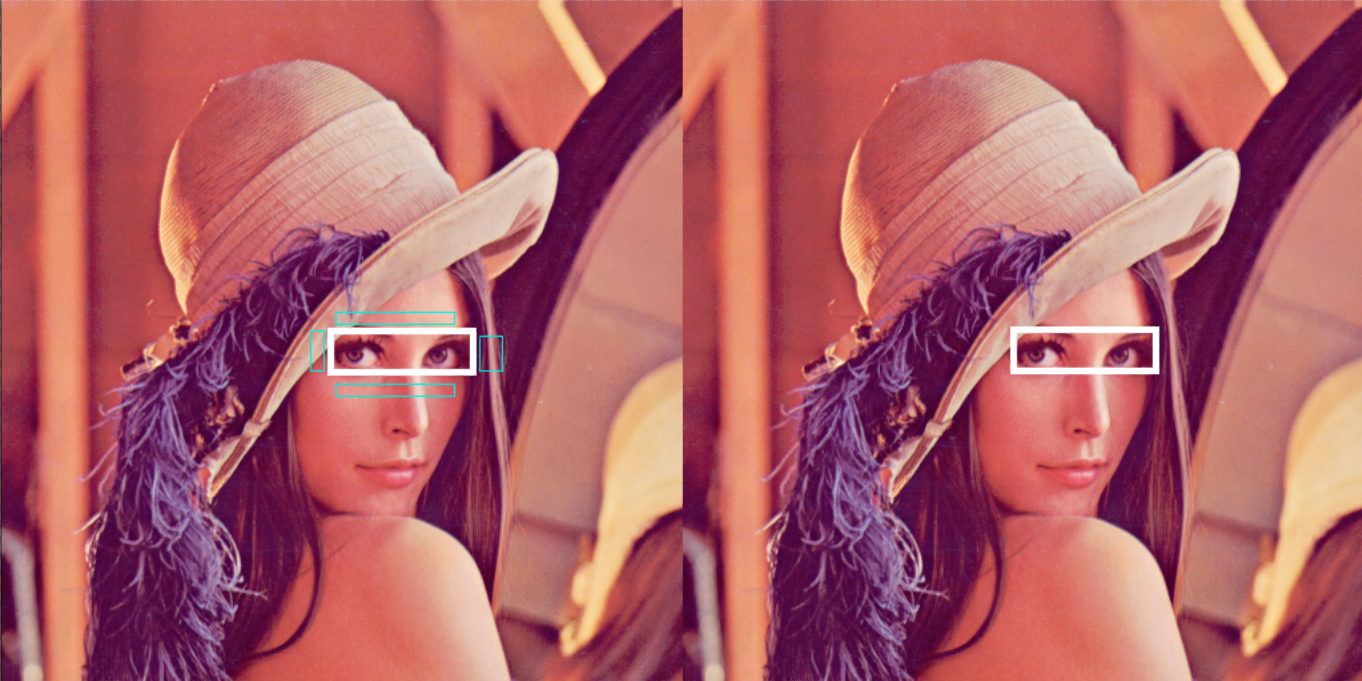
\includegraphics[width=\textwidth]{Images/Vision/Registration.PNG}\\
    \textit{Exemple de registration}\\
\end{center}

Sur l'image ci-dessus, la mise en correspondance des yeux sur l'image de gauche à comme valeur ajouter les pixels dans les rectangles bleu. Ainsi la recherche sera plus fructueuse et permettra d'identifier automatiquement les pixels en commun.\\

Cette technique consiste à faire: \sqrt{\sum((R1-R2)^2+(G1-G2)^2+(B1-B2)^2)}\\

Dès lors, le calcul de distance peut s'automatiser, par exemple en calculant avec un filtre sur l'image pour délimiter, tel un seuil, entre le plus haut pixel et le plus bas.


\subsection{Programmation}

Pour calibrer deux caméra, j'ai utilisé dans un premier temps la webcam de mon ordinateur portable (résolution: 640x480) et une caméra externe Logitech C550 (résolution réduite pour l'exercice: 640x480).\\

Pour le placement des caméras, j'ai du me baser par rapport à la webcam et donc placer la caméra externe à hauteur (quasi) équivalent et à environ 20cm horizontalement, pour ameriorer la calibration.\\

Voici un schéma du montage:

\begin{center}
    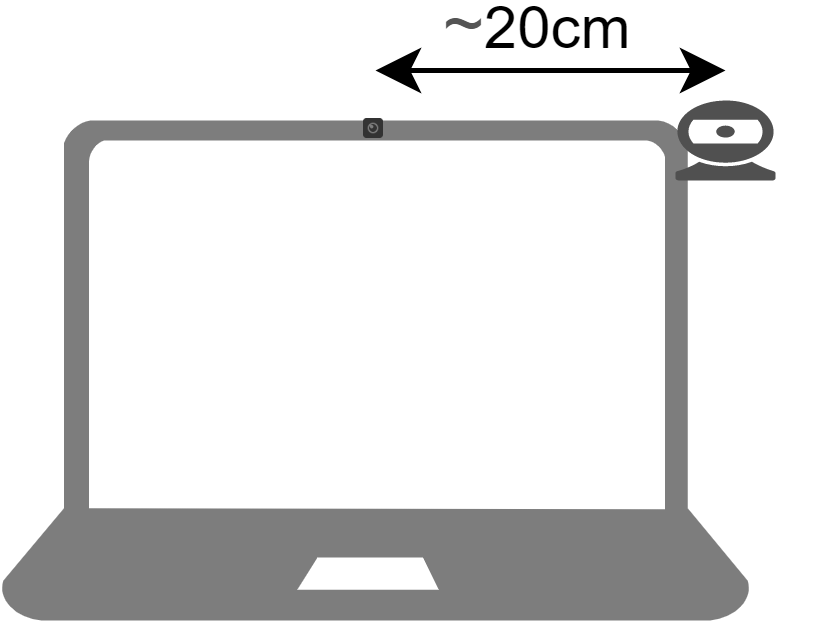
\includegraphics[width=0.5\textwidth]{Images/WCs.PNG}\\
    \textit{Positionnement des caméras de test}\\ 
\end{center}

\subsubsection{Calibration des caméras}

Grâce au bouquin \textit{Learning OpenCV: Computer Vision with the OpenCV Library by Gary Bradski and Adrian Kaehler}, le site web d'OpenCV et leur github, j'ai pu trouver explications et des programmes pour réaliser la calibration.\\

Le programme de calibration stéréo se trouve section \ref{stereo_calib.cpp}, nous permet de générer les paramètres intrinsèques et extrinsèques.  \\

Pour exécuter ce programme, je dois le compiler. Pour cela, j'ai utilisé un CMakeList.txt (permet d'exécuter un ensemble d'action). J'ai trouvé cette utilisation plus agréable que la commande g++... (qui est très longue).

Le CMakeList.txt est composé de:


\begin{minted}[
        baselinestretch=1.4,
        bgcolor=LightGray,
        fontsize=\footnotesize]
        {c++}
        
cmake_minimum_required(VERSION 3.1)
project(stereo_calib)
find_package(OpenCV REQUIRED)
add_executable(stereo_calib ../dev/stereo_calib.cpp)
target_link_libraries(stereo_calib ${OpenCV_LIBS})

\end{minted}

Après création du fichier, j'exécute "\textit{cmake .}" et "\textit{make}".

\begin{minted}[
        baselinestretch=1.4,
        bgcolor=LightGray,
        fontsize=\footnotesize]
        {c++}
$ cmake .
-- Configuring done
-- Generating done
-- Build files have been written to: /home/maxime/WalkersVision/test/cmake

$ make
[100%] Built target stereo_calib

\end{minted}

J'ai accès à mon programme, que je lance avec argument la largeur de mon plateau d'échec et sa hauteur (8x6) ainsi que le nombre d'instantanée que je souhaite (15).

\begin{minted}[
        baselinestretch=1.4,
        bgcolor=LightGray,
        fontsize=\footnotesize]
        {c++}
./stereo_calib -h=6 -w=8 -n=15
\end{minted}

Dans un premier temps, le programme va détecter les chessboard (plateau d'échec) pour nous afficher que tout marche. Si rien n'est affiché c'est que nous avons mal renseigner les arguments. \\

\begin{center}
    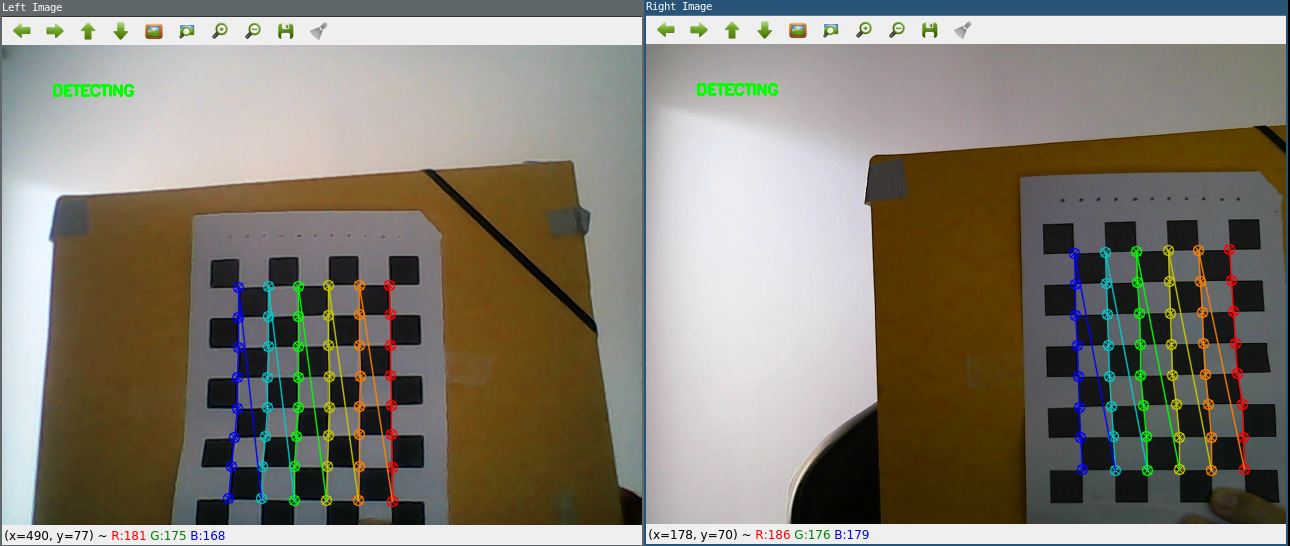
\includegraphics[width=\textwidth]{Images/Code/PhaseDetect.png}\\
    \textit{Phase de détection}
\end{center}

Tout ce passe bien, nous remarquons qu'il détecte bien notre chessboard. Pour afficher ce résultat sur l'image, le programme rentre dans la fonction \textit{calibrateFromeSavedImages()} et utilise une autre fonction: \textit{findChessboardCornersAndDraw()}. Cette dernière fonction à besoin de l'image de gauche et l'image de droite et va les traités séparément. Pour l'instant aucun stéréo n'est imaginé. La fonction \textit{findChessboardCornersAndDraw()} va modifier l'espace de couleur des images pour en venir en niveau de gris. Puis utilise la fonction \textit{findChessboardCorners()} qui va lire l'image pour trouver la position intérieur des coins du chessboard et afficher des ronds liés avec la fonction \textit{drawChessboardCorners()}. Dès lors, les images sont affichés à l'écran.\\

A la fin de chaque traitement d'images, ces images (en espace de couleur gris), sont enregistré dans le répertoire courant (car vous n'avons pas indiqué de chemin autre).\\

Le programme va prendre des photos lorsque le chessboard est bien détecté pour pouvoir appliquer les fonctions. Si le chessboard n'est pas reconnu, le programme laisse tourner le flux vidéo.\\

\begin{center}
    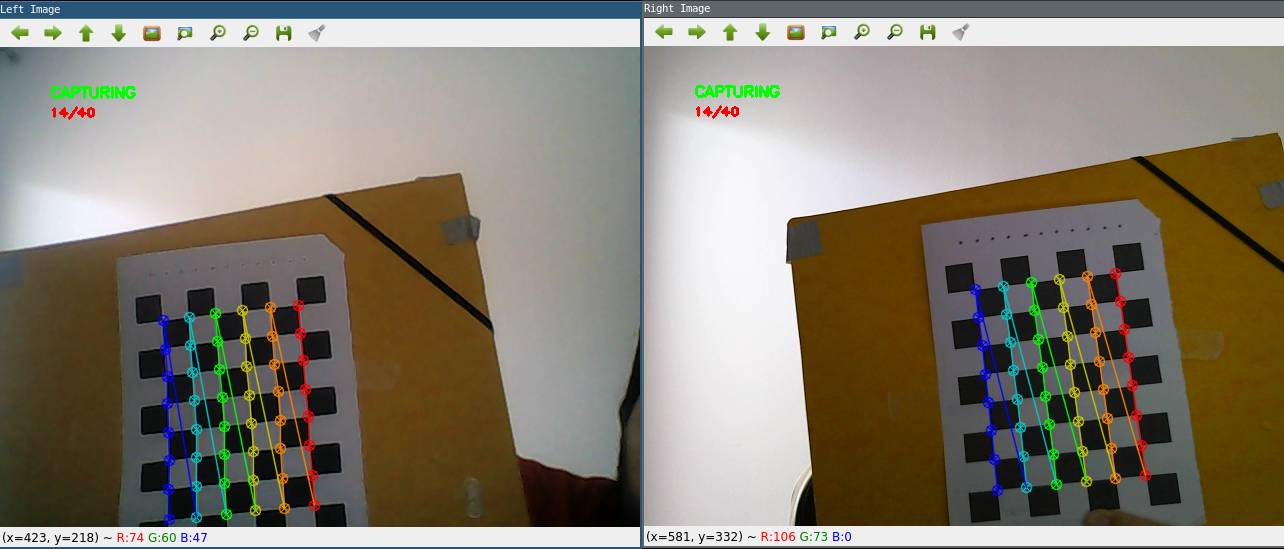
\includegraphics[width=\textwidth]{Images/Code/PhaseCapt.png}\\
    \textit{Phase de capture de photo avec chessboard}
\end{center}

Le suite du programme traite la calibration stéréo via la fonction \textit{calibrateStereoCamera()}. Cette fonction débute par l'apprentissage de pixel. Celle-ci initialise un vecteur de vecteur à 3 floats qui va recevoir chaque valeurs de pixel. \newline
Ensuite, l'utilisation des fonctions \textit{stereoCalibrate()} permet d'obtenir les paramètres intrinsèques et extrinsèques. Ultérieurement, le programme créer un fichier pour chaque paramètres est inscrit les données dedans, tel que les matrices de caméra, matrice de rotation, translation...
Le résultat des paramètres intrinsèques ce trouve page \pageref{Intrinsèques.yml}. Le résultat des paramètres extrinsèque ce trouve page \pageref{Extrinsèques.yml}. \newline
Par la suite, l'exécution de la fonction \textit{stereoRectify()}, \textit{initUndistortRectifyMap()}  permet de faire une géométrie épipôlaire.

\begin{center}
    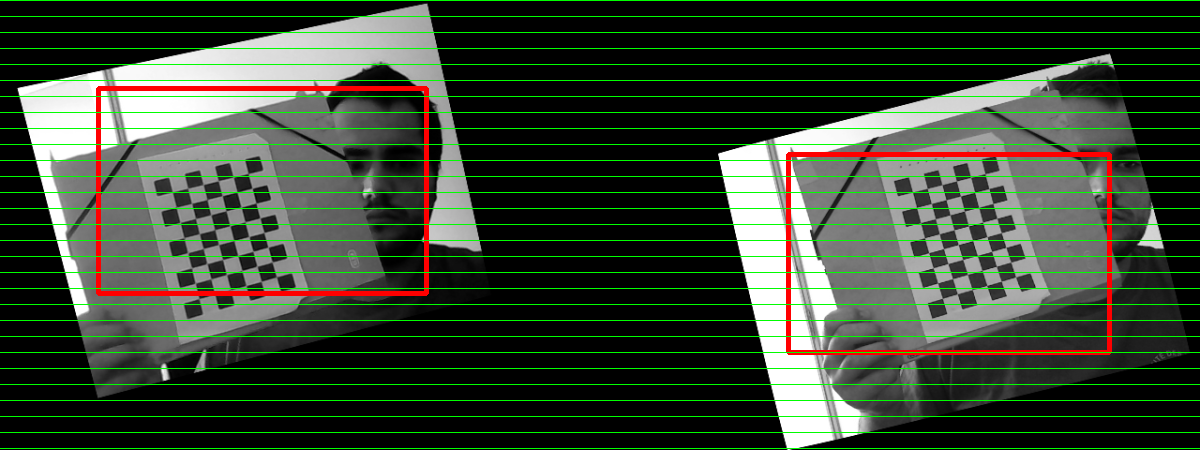
\includegraphics[width=\textwidth]{Images/epipol.png}\\
    \textit{Rectification des images avec géométrie épipolaire}\\
    \end{center}
    
    Le programme permet aussi de faire du temps différé. C'est à dire, nous donnons au programme l'emplacement de(s) image(s) déjà enregistré, le programme les charges et les traites comme précédemment.

\subsection{Disparité}

La disparité est une information importante car elle nous donner la distance entre le point d'une image et le même point sur une autre image. Voici l'explication en image:

\begin{center}
    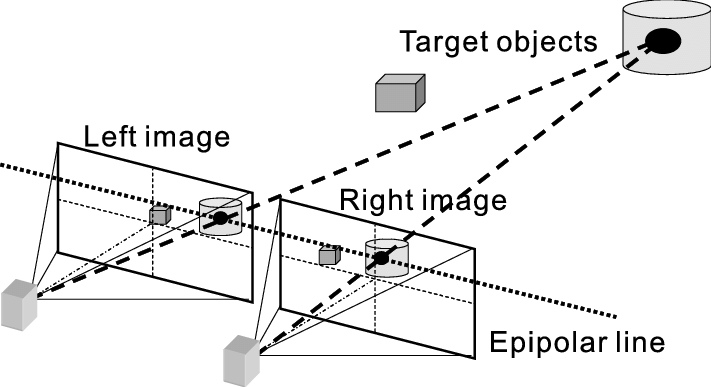
\includegraphics[width=0.8\textwidth]{Images/Binocular-stereo-vision.png}\\
    Voir bibliographie page  \pageref{biblio} - \cite{article}
\end{center}

Sur l'image de droite, l'objet n'a pas le même emplacement que sur l'image de gauche car la vue n'est pas sur la même coordonnée horizontal. Cela dit, l'objet ce trouve sur la même ligne épipolaire.\\

Voici un résultat de calcul de disparité par programmation. Le code ce trouve page \pageref{disparite}
\begin{center}
    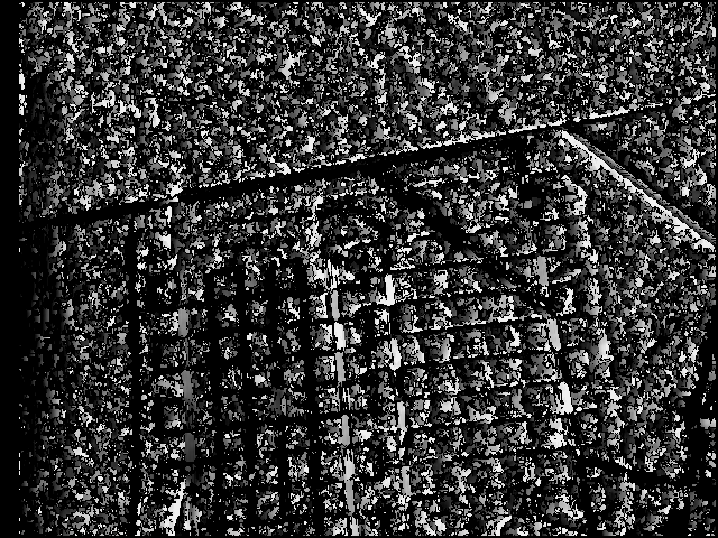
\includegraphics[width=0.6\textwidth]{Images/Code/Disparity.png}
\end{center}

Plus le pixel est clair, plus la disparité est grande. Cela s'interprète, vu précédemment, que les pixels ne sont pas affichés au même endroit sur les images.

\subsection{Conclusion}

Pour conclure cette section, grâce aux explications de mon tuteur, j'ai compris la façon dont est traité une image de façon mathématique et informatique, avec l'aide de support en plus tel que le livre de la librairie OpenCV. J'ai compris que le monde de la vision par ordinateur est un vaste domaine très intéressant et addictif. L'utilisation du langage de programmation C/C++ m'a beaucoup appris.



\newpage
\section{Dimensionnement des caméras}

Dans le cadre du projet, j'ai dû faire un dimensionnement de caméras. Ces caméras sont celle qui seront installer sur la place de Béziers.\\

Les caméras doivent répondre à plusieurs problématiques:
\begin{itemize}
    \item[$\bullet$] Voir toute la place
    \begin{itemize}
        \item[$\bullet$] Jour / Nuit
        \item[$\bullet$] Champ de profondeur
    \end{itemize}
    \item[$\bullet$] Résistance :
    \begin{itemize}
        \item[$\bullet$] Climat
        \item[$\bullet$]Vandalisme
    \end{itemize}
\end{itemize}

La commande à pour contrainte d'être acheté via le site web: \href{eneo-security.com}{eneo-security.com}\newline

Avec les problématique, ce fournisseur offres de bonnes solutions. Par la suite, j'ai dû faire un choix et donc un comparatif des offres pour ne pas avoir de caméras trop puissantes pour notre utilité ou inversement.  (Voir comparatif des caméras page: \pageref{Comparatif.pdf})

Via ce document, j'ai pu remarquer que des caméras n'avaient pas de protection anti-vandalisme. Donc nous pouvons directement sélectionner réduire le choix à (en référence): \begin{itemize}
    \item[$\bullet$] 220149
    \item[$\bullet$] 220083
    \item[$\bullet$] 219808
    \item[$\bullet$] 219026
    \item[$\bullet$] 216602
    \item[$\bullet$] 214557\\
\end{itemize}

Après analyse, la caméra (ref: 216602) propose  une qualité d'image, un flux de streaming, un capteur, sensibilité à la lumière, une MOD, angle d'image, focale dès plus compatible avec notre application. De plus, l'alimentation en plus de Ethernet (POE) est disponible. De ce fait, nous devons acheter un switch en plus qui fourni du POE. Notre besoin pour le switch est d'alimenter deux caméras, pas besoin de prendre un switch 24/48 ports.

\begin{center}
    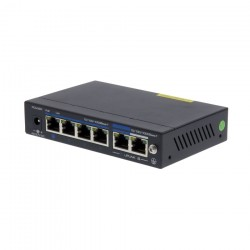
\includegraphics[width=0.4\textwidth]{Dimensionnement/SWPOE.jpg}\\
    \textit{Switch IAD-5SG1004MUA - Eneo}\\
\end{center}
\underline{Caractéristiques}:
\begin{itemize}
    \item[\bullet] Gigabit PoE switch, Desktop
    \item[\bullet] 2x Ports Gigabit Uplink/PD RJ45
    \item[\bullet] Port PD pour alimentation par 60W PoE Injector
    \item[\bullet] 4x Ports 10/100/1000 PoE, IEEE 802.3af/at
    \item[\bullet] Jusqu'à 30W par port, max. ≤60W au total
    \item[\bullet] Protection contre les surtensions IEC61000-4-5 (6KV)
    \item[\bullet] Le mode CCTV permet une transmission jusqu'à 250m @ 10Mbps
    \item[\bullet] Gamme de température : -10°C à +45°C
    \item[\bullet] Alimentation 60W contenu dans la livraison
    \item[\bullet] Power supply included\\ 
\end{itemize}
Dès la réception et lecture de la documentation, nous avons installer avec mon tuteur le matériel pour le tester avant la mise en place.
\begin{center}
    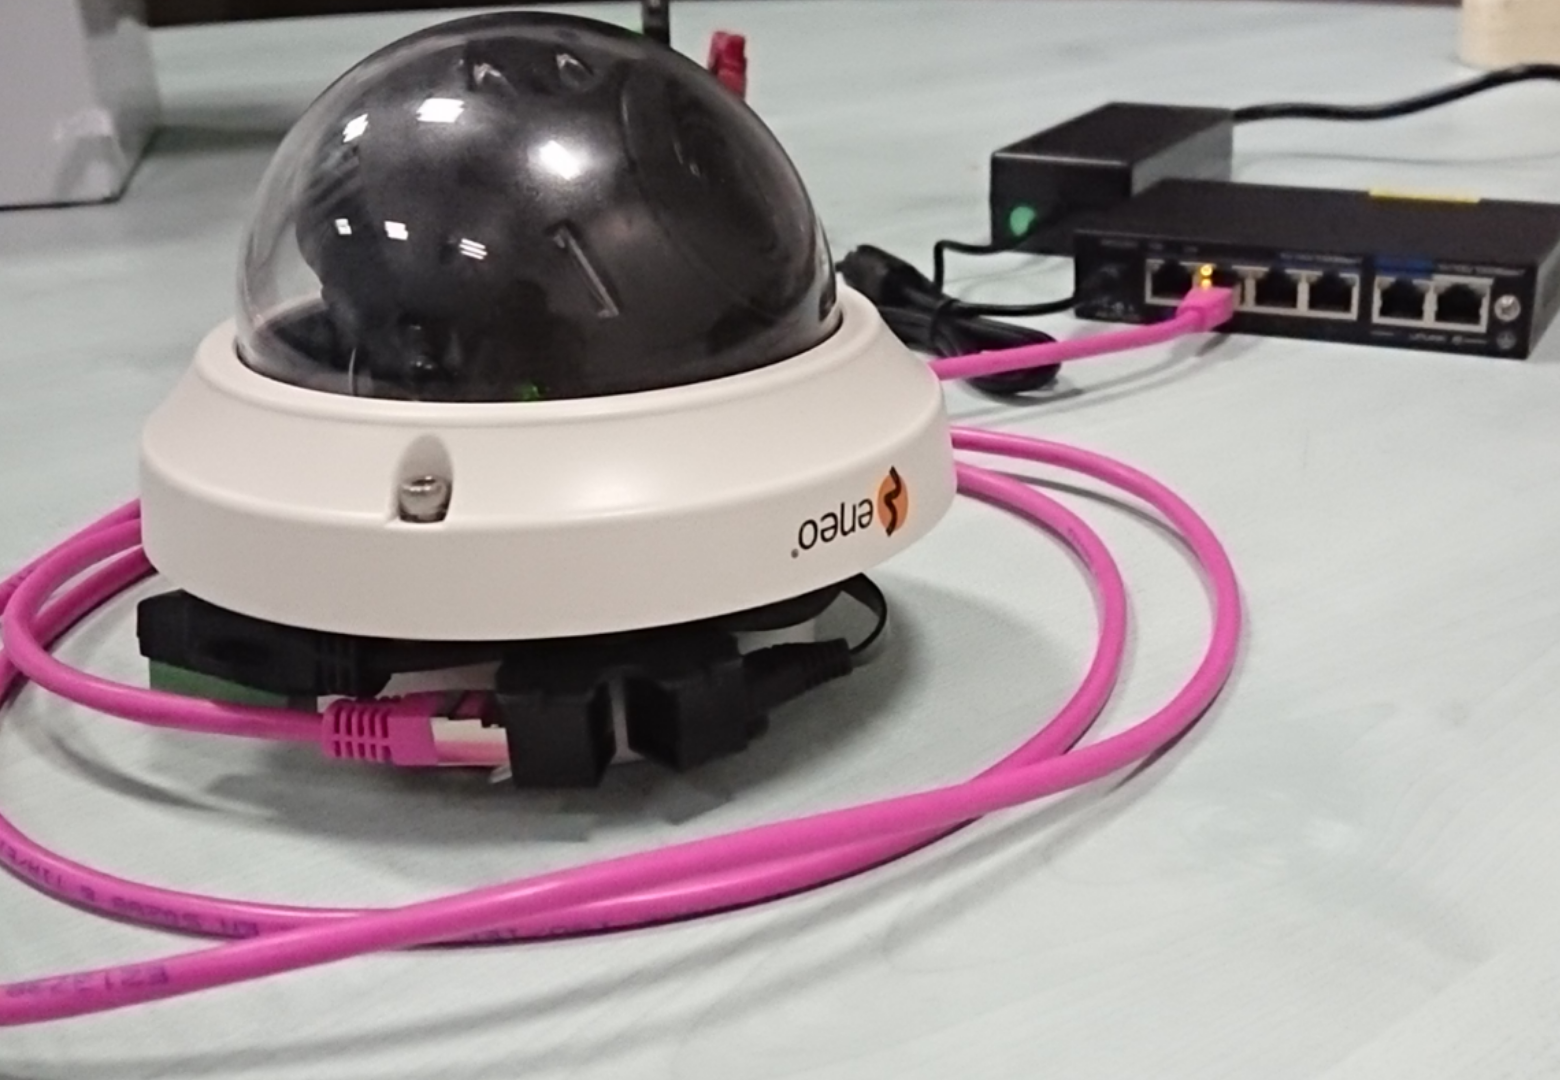
\includegraphics[width=0.6\textwidth]{Dimensionnement/camsw.png}\\
    \textit{Installation caméra/switch}\\
\end{center}

Via un navigateur web, j'ai pu interagir avec l'interface de la caméra:
\begin{center}
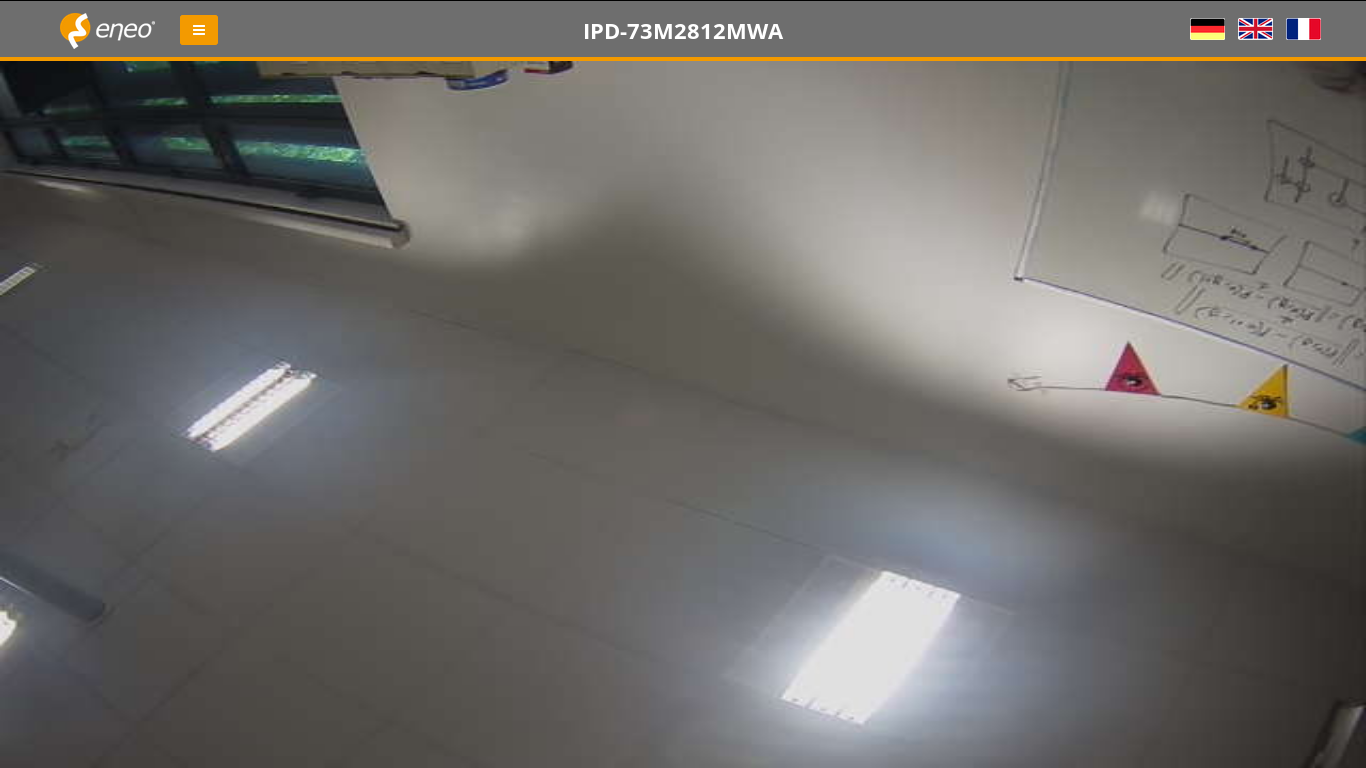
\includegraphics[width=\textwidth]{Cameras/WebSiteView.png}\\
\textit{Vue de la caméra via interface web}\\
\end{center}

Notre but étant de traiter les images de la caméra via un ordinateur distant, nous devons transiter ces images. Par curiosité, avant de regarder les paramètres dans le site web, j'ai scanné les ports de la caméra connecté sur le switch. J'ai remarqué un port que je ne connaissais pas et il se trouve que c'est utilisé pour du \textit{RTSP} (Real Time Streaming Protocol - \textbf{rfc2326}). \\

Dans un premier temps, l'objectif est de recevoir les images de la caméra sur l'ordinateur distant. Pour cela, nous allons utiliser l'outil \textit{gstreamer}. A partir de celui-ci, pour la suite il sera possible de lire le flux vidéo.

\newpage
\section{Conclusion du stage}

Ce stage m'a permis de me rendre compte de mes difficultés en anglais, en programmation et le manque de travail de mes connaissances en mathématiques. Le tuteur d'entreprise a su me guider pour que je réussisse.\\

De plus, j'ai découvert un nouveau monde dans l'informatique. Très intéressant. Qui me donne envie de continuer à m'exercer dessus. J'aurais aimé continuer et finaliser la mission. Je compte continuer de mon côté.\\

Pour finir, c'était une très bonne expérience, très enrichissante. La recherche sur le net, dans les livres, les publications, questions au tuteur et aux enseignants chercheurs présent sur les lieux du stage m'ont permis d'apprendre beaucoup de la communauté du traitement de la vision par ordinateur ainsi que d'apprendre sur le domaine.


\newpage
\section{Codes annexes}

\subsection{Calibration stéréo}
\label{stereo_calib.cpp}
\begin{minted}[
    baselinestretch=1.4,
    bgcolor=lightgray,
    fontsize=\footnotesize]
{c++}

#include <opencv2/calib3d/calib3d.hpp>
#include <opencv2/imgproc/imgproc.hpp>
#include <opencv2/highgui/highgui.hpp>
#include <opencv2/imgcodecs.hpp>
#include <iostream>
#include <stdlib.h>

// Definition du temps entre 2 capture (2 sec) 
#define timeGap 3000000000U 

using namespace cv;
using namespace std;

static void help() {
    cout<<"/******** HELP *******/\n";
    cout << "\nThis program helps you to calibrate the stereo cameras.\n This program
    generates intrinsics.yml and extrinsics.yml which can be used in Stereo Matching
    Algorithms.\n";
    cout<<"It also displays the rectified image\n";
    cout<<"\nKeyboard Shortcuts for real time (ie clicking stereo image at run
    time):\n";
    cout<<"1. Default Mode: Detecting (Which detects chessboard corners in real
    time)\n";
    cout<<"2. 'c': Starts capturing stereo images (With 2 Sec gap, This can be changed
    by changing 'timeGap' macro)\n";
    cout<<"3. 'p': Process and Calibrate (Once all the images are clicked you can press
    'p' to calibrate)";
    cout<<"\nType ./stereo_calib --help for more details.\n";
    cout<<"\n/******* HELP ENDS *********/\n\n";
}

enum Modes { DETECTING, CAPTURING, CALIBRATING};
Modes mode = DETECTING;
int noOfStereoPairs;
int stereoPairIndex = 0, cornerImageIndex=0;
int goIn = 1;
Mat _leftOri, _rightOri;
int64 prevTickCount;
vector<Point2f> cornersLeft, cornersRight;
vector<vector<Point2f> > cameraImagePoints[2];
Size boardSize;

string prefixLeft;
string prefixRight;
string postfix;
string dir;

int calibType;

Mat displayCapturedImageIndex(Mat);
Mat displayMode(Mat);
bool findChessboardCornersAndDraw(Mat, Mat);
void displayImages();
void saveImages(Mat, Mat, int);
void calibrateStereoCamera(Size);
void calibrateInRealTime(int, int);
void calibrateFromSavedImages(string, string, string, string);

Mat displayCapturedImageIndex(Mat img) {
    std::ostringstream imageIndex;
    imageIndex<<stereoPairIndex<<"/"<<noOfStereoPairs;
    putText(img, imageIndex.str().c_str(), Point(50, 70), FONT_HERSHEY_PLAIN, 0.9,
    Scalar(0,0,255), 2);
    return img;
}

Mat displayMode(Mat img) {
    String modeString = "DETECTING";
    if (mode == CAPTURING) {
        modeString="CAPTURING";
    }
    else if (mode == CALIBRATING) {
        modeString="CALIBRATED";
    }
    putText(img, modeString, Point(50,50), FONT_HERSHEY_SIMPLEX, 0.5, Scalar(0,255,0),
    2);
    if (mode == CAPTURING) {
        img = displayCapturedImageIndex(img);
    }
    return img;
}

// Pour trouver et afficher le chessbord
bool findChessboardCornersAndDraw(Mat inputLeft, Mat inputRight) {
    _leftOri = inputLeft; // Image source gauche 
    _rightOri = inputRight; // Image source droite
    bool foundLeft = false, foundRight = false;
    cvtColor(inputLeft, inputLeft, COLOR_BGR2GRAY); // Passage img en gris
    cvtColor(inputRight, inputRight, COLOR_BGR2GRAY); // Passage img en gris
    foundLeft = findChessboardCorners(inputLeft, boardSize, cornersLeft,
    CALIB_CB_ADAPTIVE_THRESH | CALIB_CB_NORMALIZE_IMAGE);
    // Recherche de coin sur SRC G
    foundRight = findChessboardCorners(inputRight, boardSize, cornersRight,
    CALIB_CB_ADAPTIVE_THRESH | CALIB_CB_NORMALIZE_IMAGE); 
    // Recherche de coin sur SRC D
    drawChessboardCorners(_leftOri, boardSize, cornersLeft, foundLeft); 
    drawChessboardCorners(_rightOri, boardSize, cornersRight, foundRight); 
    _leftOri = displayMode(_leftOri);
    _rightOri = displayMode(_rightOri);
    if (foundLeft && foundRight) {
        return true;
    }
    else {
        return false;
    }
}

void displayImages() {
    imshow("Left Image", _leftOri);
    imshow("Right Image", _rightOri);
}

// Sauvegarder les images sur le disque
void saveImages(Mat leftImage, Mat rightImage, int pairIndex) {
    cameraImagePoints[0].push_back(cornersLeft);
    cameraImagePoints[1].push_back(cornersRight);
    if (calibType == 1) {
        cvtColor(leftImage, leftImage, COLOR_BGR2GRAY);
        cvtColor(rightImage, rightImage, COLOR_BGR2GRAY);
        std::ostringstream leftString, rightString;
        leftString<<dir<<"/"<<prefixLeft<<pairIndex<<"."<<postfix;
        rightString<<dir<<"/"<<prefixRight<<pairIndex<<"."<<postfix;
        imwrite(leftString.str().c_str(), leftImage);
        imwrite(rightString.str().c_str(), rightImage);
    }
}
//Calibrage du stereo
void calibrateStereoCamera(Size imageSize) {
    vector<vector<Point3f> > objectPoints;
    objectPoints.resize(noOfStereoPairs);
    // Pour le chaque images
    for (int i=0; i<noOfStereoPairs; i++) {
        for (int j=0; j<boardSize.height; j++) {
            for (int k=0; k<boardSize.width; k++) {
                // Multiplication de j et k par 0.018 (en cm)
                // pour donner la taille d'un carré de la 
                // planche de calibration. Ainsi le resultat
                // donnera les valeurs ajusté à la réalité.
                // Coord: X,Y,Z (Z=0.0)
                objectPoints[i].push_back(Point3f(float(j*0.02),float(k*0.02),0.0)); 
            }
        }
    }
    Mat cameraMatrix[2], distCoeffs[2];
    cameraMatrix[0] = Mat::eye(3, 3, CV_64F);
    cameraMatrix[1] = Mat::eye(3, 3, CV_64F);
    Mat R, T, E, F;
    double rms = stereoCalibrate(objectPoints, cameraImagePoints[0],
    cameraImagePoints[1],
                                 cameraMatrix[0], distCoeffs[0],
                                 cameraMatrix[1], distCoeffs[1],
                                 imageSize, R, T, E, F,
                                 CALIB_FIX_ASPECT_RATIO +
                                 CALIB_ZERO_TANGENT_DIST +
                                 CALIB_SAME_FOCAL_LENGTH +
                                 CALIB_RATIONAL_MODEL +
                                 CALIB_FIX_K3 + CALIB_FIX_K4 + CALIB_FIX_K5,
                                 TermCriteria(TermCriteria::COUNT+TermCriteria::EPS,
                                 100, 1e-5) );
    cout<<"RMS Error: "<<rms<<"\n";
    double err = 0;
    int npoints = 0;
    vector<Vec3f> lines[2];
    for(int i = 0; i < noOfStereoPairs; i++ )
    {
        int npt = (int)cameraImagePoints[0][i].size();
        Mat imgpt[2];
        for(int k = 0; k < 2; k++ )
        {
            imgpt[k] = Mat(cameraImagePoints[k][i]);
            undistortPoints(imgpt[k], imgpt[k], cameraMatrix[k], distCoeffs[k], Mat(),
            cameraMatrix[k]);
            computeCorrespondEpilines(imgpt[k], k+1, F, lines[k]);
        }
        for(int j = 0; j < npt; j++ )
        {
            double errij = fabs(cameraImagePoints[0][i][j].x*lines[1][j][0] +
                                cameraImagePoints[0][i][j].y*lines[1][j][1] +
                                lines[1][j][2]) +
            fabs(cameraImagePoints[1][i][j].x*lines[0][j][0] +
                 cameraImagePoints[1][i][j].y*lines[0][j][1] + lines[0][j][2]);
            err += errij;
        }
        npoints += npt;
    }
    cout << "Average Reprojection Error: " <<  err/npoints << endl;
    FileStorage fs("intrinsics.yml", FileStorage::WRITE);
    if (fs.isOpened()) {
        fs << "M1" << cameraMatrix[0] << "D1" << distCoeffs[0] <<
        "M2" << cameraMatrix[1] << "D2" << distCoeffs[1];
        fs.release();
    }
    else
        cout<<"Error: Could not open intrinsics file.";
    Mat R1, R2, P1, P2, Q;
    Rect validROI[2];
    stereoRectify(cameraMatrix[0], distCoeffs[0], cameraMatrix[1], distCoeffs[1],
    imageSize, R, T, R1, R2, P1, P2, Q, CALIB_ZERO_DISPARITY, 1, imageSize,
    &validROI[0], &validROI[1]);
    fs.open("extrinsics.yml", FileStorage::WRITE);
    if (fs.isOpened()) {
        fs << "R" << R << "T" << T << "R1" << R1 << "R2" << R2 << "P1" << P1 
        << "P2" << P2 << "Q" << Q;
        fs.release();
    }
    else
        cout<<"Error: Could not open extrinsics file";
    bool isVerticalStereo = fabs(P2.at<double>(1, 3)) > fabs(P2.at<double>(0, 3));
    Mat rmap[2][2];
    initUndistortRectifyMap(cameraMatrix[0], distCoeffs[0], R1, P1, imageSize,
    CV_16SC2, rmap[0][0], rmap[0][1]);
    initUndistortRectifyMap(cameraMatrix[1], distCoeffs[1], R2, P2, imageSize, 
    CV_16SC2, rmap[1][0], rmap[1][1]);
    Mat canvas;
    double sf;
    int w, h;
    if (!isVerticalStereo) {
        sf = 600./MAX(imageSize.width, imageSize.height);
        w = cvRound(imageSize.width*sf);
        h = cvRound(imageSize.height*sf);
        canvas.create(h, w*2, CV_8UC3);
    }
    else {
        sf = 300./MAX(imageSize.width, imageSize.height);
        w = cvRound(imageSize.width*sf);
        h = cvRound(imageSize.height*sf);
        canvas.create(h*2, w, CV_8UC3);
    }
    String file;
    namedWindow("rectified");
    for (int i=0; i < noOfStereoPairs; i++) {
        for (int j=0; j < 2; j++) {
            if (j==0) {
                file = prefixLeft;
            }
            else if (j==1) {
                file = prefixRight;
            }
            ostringstream st;
            st<<dir<<"/"<<file<<i+1<<"."<<postfix;
            Mat img = imread(st.str().c_str()), rimg, cimg;
            remap(img, rimg, rmap[j][0], rmap[j][1], INTER_LINEAR);
            cimg=rimg;
            Mat canvasPart = !isVerticalStereo ? canvas(Rect(w*j, 0, w, h)) :
            canvas(Rect(0, h*j, w, h));
            resize(cimg, canvasPart, canvasPart.size(), 0, 0, INTER_AREA);
            Rect vroi(cvRound(validROI[j].x*sf), cvRound(validROI[j].y*sf),
                      cvRound(validROI[j].width*sf), cvRound(validROI[j].height*sf));
            rectangle(canvasPart, vroi, Scalar(0,0,255), 3, 8);
        }
        if( !isVerticalStereo )
            for(int j = 0; j < canvas.rows; j += 16 )
                line(canvas, Point(0, j), Point(canvas.cols, j), 
                Scalar(0, 255, 0), 1, 8);
        else
            for(int j = 0; j < canvas.cols; j += 16 )
                line(canvas, Point(j, 0), Point(j, canvas.rows), 
                Scalar(0, 255, 0), 1, 8);
        imshow("rectified", canvas);
    }
}

void calibrateInRealTime(int cam1, int cam2) {
    VideoCapture camLeft(cam1), camRight(cam2);
    if (!camLeft.isOpened() || !camRight.isOpened()) {
        cout<<"Error: Stereo Cameras not found or there is some 
        problem connecting them. Please check your cameras.\n";
        exit(-1);
    }
    Mat inputLeft, inputRight, copyImageLeft, copyImageRight;
    bool foundCornersInBothImage = false;
    for( ; ; ) {
        camLeft>>inputLeft;
        camRight>>inputRight;
        if ((inputLeft.rows != inputRight.rows) || (inputLeft.cols != 
        inputRight.cols)) 
        {
            cout<<"Error: Images from both cameras are not of some size. Please check 
            the size of each camera.\n";
            exit(-1);
        }
        inputLeft.copyTo(copyImageLeft);
        inputRight.copyTo(copyImageRight);
        foundCornersInBothImage = findChessboardCornersAndDraw(inputLeft,
        inputRight);
        if (foundCornersInBothImage && mode == CAPTURING &&
        stereoPairIndex<noOfStereoPairs) {
            int64 thisTick = getTickCount();
            int64 diff = thisTick - prevTickCount;
            if (goIn==1 || diff >= timeGap) {
                goIn=0;
                saveImages(copyImageLeft, copyImageRight, ++stereoPairIndex);
                prevTickCount = getTickCount();
            }
        }
        displayImages();
        if (mode == CALIBRATING) {
            calibrateStereoCamera(inputLeft.size());
            waitKey();
        }
        char keyBoardInput = (char)waitKey(50);
        if (keyBoardInput == 'q' || keyBoardInput == 'Q') {
            exit(-1);
        }
        else if(keyBoardInput == 'c' || keyBoardInput == 'C') {
            mode = CAPTURING;
        }
        else if (keyBoardInput == 'p' || keyBoardInput == 'P') {
            mode = CALIBRATING;
        }
    }
}

void calibrateFromSavedImages(string dr, string prel, string prer, string post) {
    Size imageSize;
    for (int i=0; i<noOfStereoPairs; i++) {
        Mat inputLeft, inputRight, copyImageLeft, copyImageRight;
        ostringstream imgIndex;
        imgIndex << i+1;
        bool foundCornersInBothImage = false;
        string sourceLeftImagePath, sourceRightImagePath;
        sourceLeftImagePath = dr+"/"+prel+imgIndex.str()+"."+post;
        sourceRightImagePath = dr+"/"+prer+imgIndex.str()+"."+post;
        inputLeft = imread(sourceLeftImagePath);
        inputRight = imread(sourceRightImagePath);
        imageSize = inputLeft.size();
        if (inputLeft.empty() || inputRight.empty()) {
            cout<<"\nCould no find image: "<<sourceLeftImagePath<<" or
            "<<sourceRightImagePath<<". Skipping images.\n";
            continue;
        }
        if ((inputLeft.rows != inputRight.rows) || (inputLeft.cols !=
        inputRight.cols)) 
        {
            cout<<"\nError: Left and Right images are not of some size. Please check
            the size of the images. Skipping Images.\n";
            continue;
        }
        inputLeft.copyTo(copyImageLeft);
        inputRight.copyTo(copyImageRight);
        foundCornersInBothImage = findChessboardCornersAndDraw(inputLeft, inputRight);
        if (foundCornersInBothImage && stereoPairIndex<noOfStereoPairs) {
            saveImages(copyImageLeft, copyImageRight, ++stereoPairIndex);
        }
        displayImages();
    }
    if(stereoPairIndex > 2) {
        calibrateStereoCamera(imageSize);
        waitKey();
    }
    else {
        cout<<"\nInsufficient stereo images to calibrate.\n";
    }
}

int main(int argc, char** argv) {
    help();
    const String keys =
    "{help| |Prints this}"
    "{h height|7|Height of the board}"
    "{w width|7|Width of the board}"
    "{rt realtime|1|Clicks stereo images before calibration. Use if you do not have
    stereo pair images saved}"
    "{n images|40|No of stereo pair images}"
    "{dr folder|.|Directory of images}"
    "{prel prefixleft|image_left_|Left image name prefix. Ex: image_left_}"
    "{prer prefixright|image_right_|Right image name postfix. Ex: image_right_}"
    "{post postfix|jpg|Image extension. Ex: jpg,png etc}"
    "{cam1|0|Camera 1 Index}"
    "{cam2|2|Camera 2 Index}";
    CommandLineParser parser(argc, argv, keys);
    if(parser.has("help")) {
        parser.printMessage();
        exit(-1);
    }
    boardSize = Size(parser.get<int>("w"), parser.get<int>("h"));
    noOfStereoPairs = parser.get<int>("n");
    prefixLeft = parser.get<string>("prel");
    prefixRight = parser.get<string>("prer");
    postfix = parser.get<string>("post");
    dir =parser.get<string>("dr");
    calibType = parser.get<int>("rt");
    namedWindow("Left Image");
    namedWindow("Right Image");
    switch (calibType) {
        case 0:
            calibrateFromSavedImages(dir, prefixLeft, prefixRight, postfix);
            break;
        case 1:
            calibrateInRealTime(parser.get<int>("cam1"), parser.get<int>("cam2"));
            break;
        default:
            cout<<"-rt should be 0 or 1. Ex: -rt=1\n";
            break;
    }
    return 0;
}

\end{minted}

\subsection{Intrinsèques.yml}
\label{Intrinsèques.yml}
\begin{minted}[
        baselinestretch=1.4,
        bgcolor=LightGray,
        fontsize=\footnotesize]
        {bash}
        
$ cat intrinsics.yml 
%YAML:1.0
---
M1: !!opencv-matrix
   rows: 3
   cols: 3
   dt: d
   data: [ 9.8710906989142154e+02, 0., 2.8138121365893630e+02, 0.,
       9.8710906989142154e+02, 2.3801545388613809e+02, 0., 0., 1. ]
D1: !!opencv-matrix
   rows: 1
   cols: 14
   dt: d
   data: [ 2.0029047342300932e-02, -2.8402240995911338e-01, 0., 0., 0.,
       0., 0., -1.3240532524068107e+00, 0., 0., 0., 0., 0., 0. ]
M2: !!opencv-matrix
   rows: 3
   cols: 3
   dt: d
   data: [ 9.8710906989142154e+02, 0., 3.0918767142390823e+02, 0.,
       9.8710906989142154e+02, 2.3417007433393971e+02, 0., 0., 1. ]
D2: !!opencv-matrix
   rows: 1
   cols: 14
   dt: d
   data: [ -6.0534709383844081e-02, 3.5168116835394517e-02, 0., 0., 0.,
       0., 0., -3.6174740105995693e+00, 0., 0., 0., 0., 0., 0. ]

\end{minted}

\subsection{Extrinsèques.yml}
\label{Extrinsèques.yml}
\begin{minted}[
        baselinestretch=1.4,
        bgcolor=LightGray,
        fontsize=\footnotesize]
        {bash}
        
$ cat extrinsics.yml 
%YAML:1.0
---
R: !!opencv-matrix
   rows: 3
   cols: 3
   dt: d
   data: [ 9.9082334299705421e-01, -1.6339643336906441e-02,
       -1.3417197556779314e-01, 1.3491940526615936e-03,
       9.9381229919569458e-01, -1.1106436711554053e-01,
       1.3515651167276421e-01, 1.0986414348180205e-01,
       9.8471446995027956e-01 ]
T: !!opencv-matrix
   rows: 3
   cols: 1
   dt: d
   data: [ 1.7114464211401462e-01, 4.2458825467741268e-02,
       7.3495078172759135e-03 ]
R1: !!opencv-matrix
   rows: 3
   cols: 3
   dt: d
   data: [ 9.6678982692080984e-01, 2.2782057412348117e-01,
       -1.1582407594484888e-01, -2.3304788503951440e-01,
       9.7188420087857208e-01, -3.3612250166102135e-02,
       1.0491002736173502e-01, 5.9488537456107958e-02,
       9.9270086132242941e-01 ]
R2: !!opencv-matrix
   rows: 3
   cols: 3
   dt: d
   data: [ 9.6973576644706772e-01, 2.4057920334995220e-01,
       4.1643609219427377e-02, -2.4227970373231017e-01,
       9.6928916869865067e-01, 4.2178816992214076e-02,
       -3.0217353171679937e-02, -5.0991708727802287e-02,
       9.9824183302860880e-01 ]
P1: !!opencv-matrix
   rows: 3
   cols: 4
   dt: d
   data: [ 6.7554769475498335e+02, 0., 3.3616869544982910e+02, 0., 0.,
       6.7554769475498335e+02, 2.3718235111236572e+02, 0., 0., 0., 1.,
       0. ]
P2: !!opencv-matrix
   rows: 3
   cols: 4
   dt: d
   data: [ 6.7554769475498335e+02, 0., 3.3616869544982910e+02,
       1.1922460988871862e+02, 0., 6.7554769475498335e+02,
       2.3718235111236572e+02, 0., 0., 0., 1., 0. ]
Q: !!opencv-matrix
   rows: 4
   cols: 4
   dt: d
   data: [ 1., 0., 0., -3.3616869544982910e+02, 0., 1., 0.,
       -2.3718235111236572e+02, 0., 0., 0., 6.7554769475498335e+02, 0.,
       0., -5.6661766004981962e+00, 0. ]


\end{minted}


\subsection{Disparité}
\label{disparite}
\begin{minted}[
    baselinestretch=1.4,
    bgcolor=lightgray,
    fontsize=\footnotesize]
{c++}
/**
 * @file SBM_Sample
 * @brief Get a disparity map of two images
 * @author A. Huaman
 */

#include <stdio.h>
#include <iostream>
#include "opencv2/calib3d/calib3d.hpp"
#include "opencv2/core/core.hpp"
#include "opencv2/highgui/highgui.hpp"

using namespace cv;

const char *windowDisparity = "Disparity";

void readme();

/**
 * @function main
 * @brief Main function
 */
int main( int argc, char** argv )
{
  if( argc != 3 )
  { readme(); return -1; }

  //-- 1. Read the images
  Mat imgLeft = imread( argv[1], IMREAD_GRAYSCALE );
  Mat imgRight = imread( argv[2], IMREAD_GRAYSCALE );
  //-- And create the image in which we will save our disparities
  Mat imgDisparity16S = Mat( imgLeft.rows, imgLeft.cols, CV_16S );
  Mat imgDisparity8U = Mat( imgLeft.rows, imgLeft.cols, CV_8UC1 );

  if( !imgLeft.data || !imgRight.data )
  { std::cout<< " --(!) Error reading images " << std::endl; return -1; }

  //-- 2. Call the constructor for StereoBM
  int ndisparities = 112;   /**< Range of disparity */
  int SADWindowSize = 5; /**< Size of the block window. Must be odd */

  Ptr<StereoBM> sbm = StereoBM::create( ndisparities, SADWindowSize );

  //-- 3. Calculate the disparity image
  sbm->compute( imgLeft, imgRight, imgDisparity16S );

  //-- Check its extreme values
  double minVal; double maxVal;

  minMaxLoc( imgDisparity16S, &minVal, &maxVal );

  printf("Min disp: %f Max value: %f \n", minVal, maxVal);

  //-- 4. Display it as a CV_8UC1 image
  imgDisparity16S.convertTo( imgDisparity8U, CV_8UC1, 255/(maxVal - minVal));
  
  namedWindow( windowDisparity, WINDOW_NORMAL );
  imshow( windowDisparity, imgDisparity8U );

  //-- 5. Save the image
  imwrite("SBM_sample.png", imgDisparity16S); 

  waitKey(0);

  return 0;
}

void readme(){ 
    std::cout << " Usage: ./SBMSample <imgLeft> <imgRight>" 
    << std::endl;
}

\end{minted}








\subsection{Comparatif des caméras}
\label{Comparatif.pdf}
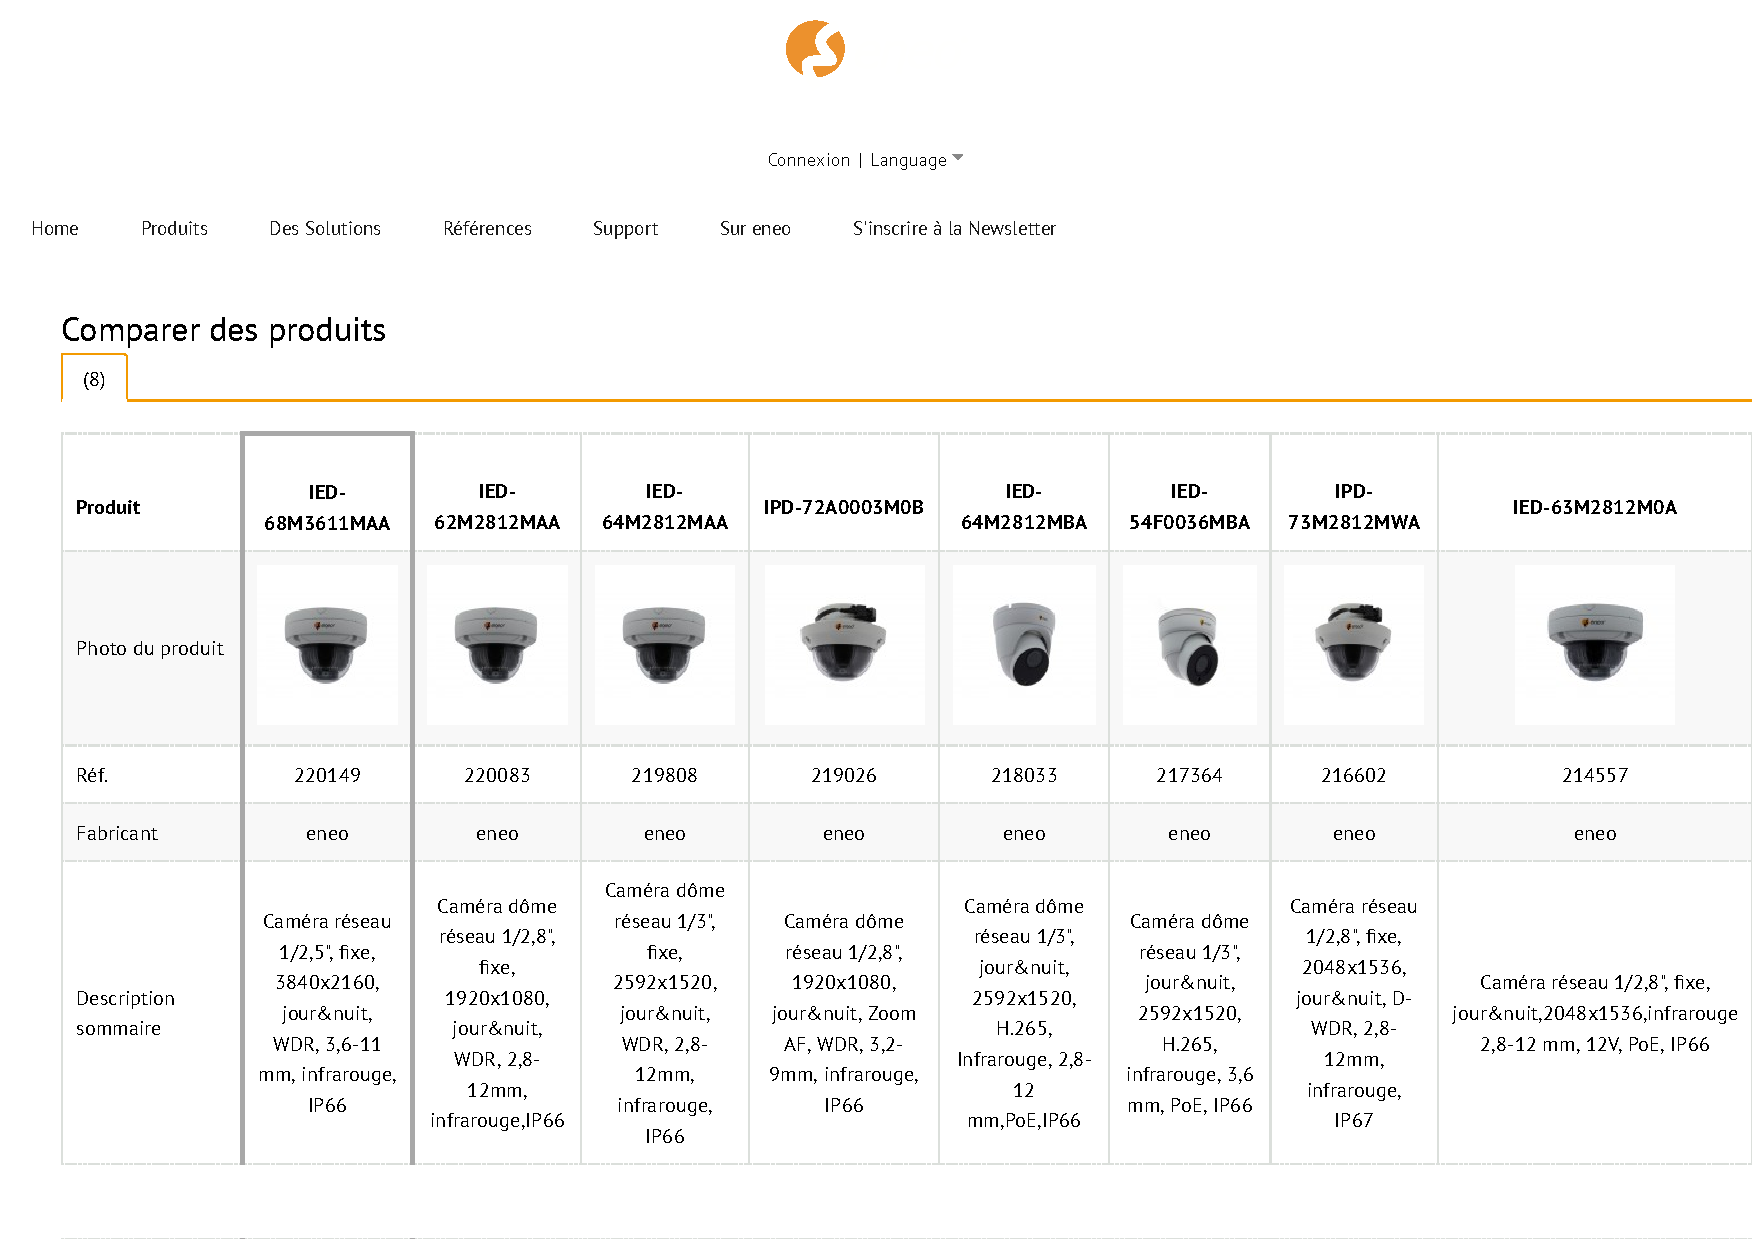
\includegraphics[width=\textwidth,page=1]{Dimensionnement/Comparatif.pdf}
\includegraphics[width=\textwidth,page=2]{Dimensionnement/Comparatif.pdf}
\includegraphics[width=\textwidth,page=4]{Dimensionnement/Comparatif.pdf}
\includegraphics[width=\textwidth,page=5]{Dimensionnement/Comparatif.pdf}
\newpage
\label{biblio}
\printbibliography[title={Bibliographie}]


































\end{document}



% Ligne de codes
\begin{minted}[
    baselinestretch=1.4,
    bgcolor=lightgray,
    fontsize=\footnotesize]
{c++}

\end{minted}



\begin{center}
    \begin{tikzpicture}
  
        \path(3.5,-2) node{u',v'};
        % Marqueur
        \draw(3,-1.75) circle (0.05);
        % Plan
        \draw[-](3,-4) -- (3,-1); 
        % Repères
        \draw[->](0,0) -- (0,2); 
        % Visu CAM
        \draw[-](0,0) -- (6,0.5);
     \end{tikzpicture}
\end{center}

$$\begin{matrix}
    
    \underbrace{\begin{bmatrix}
        u'\\
    \end{bmatrix}}_{\text{Coord. H. pixel}}
    =
    \underbrace{\begin{bmatrix}
        \alpha f \\
    \end{bmatrix}}_{\text{Matrice de projection}}
    \underbrace{\begin{bmatrix}
        X\\
    \end{bmatrix}}_{\text{Coord. 3D du point}}
\end{matrix}$$


